\documentclass[journal]{IEEEtran}

% Useful packages
\usepackage{cite}
\usepackage{graphicx}
\usepackage{amsmath,amssymb,amsfonts}
\usepackage{bm}
\usepackage{booktabs}
\usepackage{textcomp}
\usepackage{xcolor}
\usepackage{url}
\usepackage[hidelinks]{hyperref}
\usepackage{float}
\usepackage{cuted}
\usepackage{caption}
% NOTE: dblfloatfix and stfloats do the same job and explicitly conflict
% ("Package dblfloatfix Error: Don't use the stfloats package!"). The original
% preamble loaded both. Keeping stfloats only.
\usepackage{stfloats}

% Range separator used in place of en dashes (e.g. 2010\rng{}2022, C1\rng{}C4).
% Change this one line to restyle every range in the paper.
\newcommand{\rng}{\ensuremath{\sim}}

% Figure placeholder: draws a labelled box until the image file exists,
% then includes the image automatically. Usage: \figplaceholder{figs/name.png}
\newcommand{\figplaceholder}[2][\linewidth]{%
  \IfFileExists{#2}{\includegraphics[width=#1]{#2}}{%
    \fbox{\parbox[c][0.55#1][c]{0.95#1}{\centering\footnotesize Figure to be added:\\[2pt]\texttt{\detokenize{#2}}}}}}

\hyphenation{op-tical net-works semi-conduc-tor Ga-bil-lon back-war-da-tion}

\begin{document}

\title{News-Augmented Latent Factor Estimation in Oil Futures Pricing: A State-Space Extension of the Gabillon Two-Factor Model}

\author{Bradley Wright}

\maketitle

\begin{abstract}
Drawing accurate oil futures curves poses an interesting challenge, shaped simultaneously by transient shocks and slow-moving expectations about long-term equilibrium. Two-factor models capture this separation and, because they are linear and Gaussian, admit a closed-form futures price that maps directly onto a state-space representation. Using these models, unobservable factors become recoverable by Kalman filtering and indiscernible parameters by maximum likelihood. This paper develops that representation to formalise a distinction that the existing literature leaves ambiguous. We show that when prices are treated as noisy indicators of latent states, news emerges in two fundamentally different roles: as a driver that shifts factor dynamics, or as a measurement that reveals an existing shock. Standard return-predictability models cannot separate these roles because both yield the same surface-level correlation between news and future prices. Estimated on a panel of eighteen nearby WTI contracts and daily news-sentiment data, the two mechanisms separate cleanly: financial news and sentiment are a mirror, not a motor. The measurement channel is overwhelmingly significant ($p = 3.6 \times 10^{-7}$), whereas the driver channel shows no statistical significance, and an unrestricted specification adds no incremental explanatory power. News measures contemporaneous shocks rather than driving next-day state transitions, a finding that survives a block-shuffled placebo control and re-estimation across contract maturities.

The price-side results share a common theme. Five times in this study, a specification that fitted better turned out not to fit better for the reason it was built:
\begin{enumerate}
    \item A free diagonal measurement-error covariance produced a profile whose shape invited a structural interpretation, yet was merely an artefact of unidentifiability.
    \item A filter appeared to beat a random walk on seventeen of eighteen contracts until the sequential updating order was reversed.
    \item A likelihood ratio of $15{,}982$ collapsed to $59.09$ once evaluated on a common observation set.
    \item An essentially-affine market price of risk, built to repair the front of the curve, delivered a large, well-identified gain that a maturity decomposition revealed accrued mostly to the deferred end.
    \item A front-exclusive fourth factor, built for the same purpose, delivered a larger gain that a back-loaded placebo matched and exceeded, showing it was not about the front.
\end{enumerate}

The constructive counterpart is sharper: a misspecified measurement variance forecasts \emph{worse than doing nothing}, and the damage grows monotonically with the degree of misspecification across $53{,}000$ observations. Filtering helps cross-sectionally (outpricing a dynamics-free curve on fourteen of eighteen held-out maturities) but hurts temporally, making our diagnostic framework the primary contribution of this study.
\end{abstract}

\begin{IEEEkeywords}
Oil futures, term structure, latent factor estimation, state-space models, Kalman filter, financial news sentiment, natural language processing, contango and backwardation, commodity risk premia.
\end{IEEEkeywords}

\tableofcontents

\section*{Nomenclature}
\addcontentsline{toc}{section}{Nomenclature}

\noindent\textit{Latent state and pricing.}

\smallskip
\begin{tabular}{@{}p{2.0cm}@{}p{5.95cm}@{}}
$S_t$            & Spot price of crude oil at time $t$ \\
$F(t,T)$         & Futures price at $t$ for delivery at $T$ \\
$\tau$           & Time to maturity, $\tau = T - t$ (years) \\
$\chi_t$         & Short-run latent factor (transient deviation) \\
$\chi_{1,t},\chi_{2,t}$ & Fast and slow transient factors in the three-factor extension (Sec.~\ref{sec:threefactor}) \\
$\xi_t$          & Long-run latent factor (equilibrium level) \\
$\bm{x}_t$       & State vector $(\chi_t,\xi_t)^{\!\top}$ \\
$\bm{z}_t$       & Augmented state $(\chi_t,\xi_t,w^\chi_t,w^\xi_t)^{\!\top}$ \\
$A(\tau)$        & Deterministic log-futures adjustment \\
$\bar{a}$        & Time-invariant part of the front-end slope \\
\end{tabular}

\smallskip
\noindent\textit{Model parameters.}

\smallskip
\begin{tabular}{@{}p{2.0cm}@{}p{5.95cm}@{}}
$\kappa$           & Short-run mean-reversion speed (per year) \\
$\kappa_1,\kappa_2$& Fast and slow reversion rates, $\kappa_1 > \kappa_2 > 0$ \\
$g$                & Log-gap parameter enforcing that ordering, $\kappa_1 = \kappa_2 + e^{g}$ \\
$\sigma_\chi$      & Short-run diffusion coefficient \\
$\sigma_1,\sigma_2$& Diffusion coefficients of $\chi_1$ and $\chi_2$ \\
$\sigma_\xi$       & Long-run diffusion coefficient \\
$\rho$             & Correlation of the two Brownian motions \\
$\mu_\xi$          & Long-run drift under $\mathbb{P}$ \\
$\mu_\xi^{*}$      & Long-run drift under $\mathbb{Q}$ \\
$\lambda_\chi$     & Short-run market price of risk \\
$\lambda_\xi$      & Long-run market price of risk, $\lambda_\xi = \mu_\xi - \mu_\xi^{*}$ \\
$\lambda_1,\lambda_2$ & Market prices of risk on $\chi_1$ and $\chi_2$ \\
$s_i$              & Measurement-error s.d.\ for contract $i$ \\
$s(\tau)$          & Smooth measurement-error curve, $\exp(a + b\tau + c\tau^{2})$ \\
$a,b,c$            & Its level, slope and curvature coefficients \\
$\nu$              & Degrees of freedom of the Student-$t$ observation density (scalar; distinct from the prediction error $\bm{\nu}_t$) \\
$\kappa_f^{\mathbb{Q}}$ & Risk-neutral rate of the front-concentrated factor, fixing its loading decay (Sec.~\ref{sec:rungs}) \\
$\kappa_f^{\mathbb{P}}$ & Its physical reversion rate, free under an affine market price of risk \\
$\Lambda$          & State-dependent coefficient of the market price of risk; $\Lambda = 0$ recovers the completely affine case \\
$\bm{\theta}$      & Full parameter vector \\
\end{tabular}

\smallskip
\noindent\textit{State-space system.}

\smallskip
\begin{tabular}{@{}p{2.0cm}@{}p{5.95cm}@{}}
$\bm{T},\bm{c}$    & Transition matrix and intercept \\
$\bm{Q}$           & State (process) noise covariance \\
$\bm{Z}_t,\bm{d}_t$& Price-channel loadings and intercept \\
$\bm{H}$           & Price-channel noise covariance \\
$\bm{v}_t,\bm{w}_t$& Measurement and state disturbances \\
$\bm{\nu}_t,\bm{S}_t$ & Prediction error and its covariance \\
$\bm{P}_t$         & Posterior state covariance (filter output) \\
$\ell(\bm{\theta})$& Exact Gaussian log-likelihood \\
$m,\,m_t$          & Contracts available; observed at $t$ \\
\end{tabular}

\smallskip
\noindent\textit{News channel.}

\smallskip
\begin{tabular}{@{}p{2.0cm}@{}p{5.95cm}@{}}
$\bm{u}_t$         & Daily news feature vector, $p$ features \\
$\bm{n}_t$         & News observation vector (measurement view) \\
$I_t$              & News intensity (article volume) \\
$\bm{B}$           & Channel-A driver loadings, $2\times p$ \\
$\bm{G}$           & Channel-M measurement loadings \\
$\bm{R}_t$         & News-channel noise covariance \\
$\gamma$           & Intensity coefficient on short-run variance \\
$\gamma_r,\gamma_v$& Release-window and lagged-volatility loadings \\
$\eta$             & Roll-window inflation of $s_i^2$ (one shared coefficient, not per-contract) \\
$\bm{G}^{\pm}$     & Asymmetric loadings on $\bm{u}^{+}_t,\bm{u}^{-}_t$ \\
$\varsigma_t^2$    & Within-day dispersion of document sentiment \\
$\Delta_\ell$      & News-to-price lead/lag in trading sessions \\
$\bm{e}_t$         & News measurement disturbance \\
$\mathrm{RV}_{t-1}$& Lagged realised volatility, the driver of $\gamma_v$ \\
$\zeta,\ \varkappa_t$ & No-trade band width; round-trip spread cost \\
\end{tabular}

\smallskip
\noindent\textit{Specifications and tests.}

\smallskip
\begin{tabular}{@{}p{2.0cm}@{}p{5.95cm}@{}}
$\mathrm{S0}$      & Baseline: prices only \\
$\mathrm{SD}$      & News as driver of factor dynamics \\
$\mathrm{SM}$      & News as measurement of innovations \\
$\mathrm{SDM}$     & Both channels, unrestricted \\
LR                 & Likelihood-ratio statistic \\
DM                 & Diebold-Mariano statistic \\
MCS                & Model Confidence Set \\
\end{tabular}
\smallskip

\section{Introduction}

\IEEEPARstart{O}{il} price dynamics remain difficult to model despite sustained academic and industry attention, owing to persistent volatility, structural breaks, and expectations that shift with events \cite{Pan2024, Li2023, Du2025}. Futures markets are shaped by temporary disturbances and by more durable (i.e., events whose impacts decay slowly across longer horizons) structural beliefs simultaneously \cite{He2024}, and the frequent transition between contango and backwardation indicates that expectations and risk premia vary across maturities rather than moving in lockstep \cite{Gorton2013, Cortazar2022}. Schwartz and Smith formalise this observation, arguing that commodity prices reflect short-run adjustment alongside genuine uncertainty about the longer-run equilibrium level \cite{SchwartzSmith2000, Lee2023}.

Multi-factor models accommodate this by admitting several distinct sources of uncertainty \cite{Pindyck1999, Ballestra2025}. In Gabillon's \cite{Gabillon1992} two-factor framework, the shape of the futures curve is jointly determined by short-run deviations and long-run equilibrium expectations. While this model simplifies the complex nature behind drawing these curves, its practical difficulty is that neither factor is easily observable to even the most exemplary financial analysts. Both must be extracted from a noisy panel of futures prices, which makes estimates sensitive to market microstructure and to structural change \cite{SchwartzSmith2000, Peters2011}.

Oil markets are, at the same time, unusually sensitive to information surrounding geopolitical developments, production policy, and macroeconomic conditions \cite{KilianMurphy2014}. A substantial literature now shows that textual data carries predictive signal for oil futures returns \cite{Pan2024} and that news-derived features contain information beyond price-based indicators \cite{Gong2022}. Advances in natural language processing make such features cheap to construct at scale \cite{Araci2019}, while recent breakthroughs in large language models enable sentiment to be extracted seamlessly from textual data. This raises an obvious question, which the existing literature has answered only for returns and volatility, not for the term structure itself.

\subsection{Research question and contribution}

\begin{quote}
\textit{Does textual news carry information about the latent short-run and long-run factors of a two-factor oil futures pricing model beyond that already contained in the futures panel?}
\end{quote}

The framing matters. Asking whether news ``improves estimation'' is not testable as stated; asking whether news carries \emph{incremental} information, relative to an explicit baseline, is. The paper makes six contributions.

\begin{enumerate}
  \item It states the closed-form futures price implied by the two-factor model and shows that the contango/backwardation distinction follows from it directly, with the sign of the short-run factor determining the front-end slope (Section~\ref{sec:twofactor}).
  \item It reconciles Gabillon's parametrisation with the Schwartz-Smith form, which are related by a change of variables and are frequently conflated (Section~\ref{sec:gabillon-relation}).
  \item It specifies two concrete mechanisms by which news enters the model, as a driver of the factor dynamics and as a second measurement of the same latent shock, each nesting the baseline as a parameter restriction and therefore testable rather than merely asserted (Section~\ref{sec:empirical}).
  \item It reports that the two mechanisms separate empirically, and in a direction the design did not presume: news measures the contemporaneous shock and does not drive the transition, at $p = 3.6\times10^{-7}$ against $p = 0.99$ (Section~\ref{sec:newsresult}). The distinction is inexpressible in a returns-prediction formulation, which is the substantive case for the state-space framing.
  \item It documents an identification failure of independent interest. With $k$ latent factors and a free diagonal measurement covariance, the likelihood is raised by pricing exactly $k$ contracts without error and absorbing the misfit into the remainder \cite{ChenScott1993}; the resulting error profile is not stably estimated, and a mechanism inferred from its shape was refuted by the panel-perturbation diagnostic that ought to have preceded it (Sections~\ref{sec:firstcontact}\rng{}\ref{sec:smoothcurve}).
  \item It sets out, and applies, an evaluation protocol that treats the random walk as the benchmark to beat, reports performance conditionally on market regime, and uses a block-shuffled placebo to guard against spurious findings.
\end{enumerate}

Part~I, comprising Sections~\ref{sec:markets}\rng{}\ref{sec:empirical}, develops the framework and design. Part~II reports the implementation and results.

% =====================================================================
\section{Oil Futures Markets and Term Structure}
\label{sec:markets}
% =====================================================================

\subsection{Economic role and price discovery}

Oil futures are standardised contracts specifying delivery of crude at a predetermined price and maturity \cite{Lee2024}. They allow participants to hedge exposure to price fluctuations \cite{HamiltonWu2014, Anthropelos2015} and, through the interaction of hedgers and speculators, support liquidity and price discovery \cite{KilianMurphy2014, Kaufmann2009}. Because they embed expectations about future prices, they carry information about the economic drivers of commodity dynamics \cite{Gorton2013, Yu2023}.

Crucially for what follows, differences \emph{between} maturities are informative in a way that any single price is not. Participants evaluating future supply, demand conditions and the associated risks will price near and deferred contracts differently \cite{HamiltonWu2014, Cortazar2022}, and the resulting cross-section provides a natural framework for separating transitory from persistent components of price variation \cite{SchwartzSmith2000}. This is the identifying variation the rest of the paper exploits.

\subsection{The cost of carry and its limits}

The term structure describes how futures prices vary with maturity \cite{Gorton2013, HamiltonWu2014}. Under the cost-of-carry relationship, the price of a contract $F(t,T)$ at time $t$ for delivery at $T$ satisfies
%
\begin{equation}
  F(t,T) = S_t \exp\bigl((r + c - y)(T - t)\bigr) ,
  \label{eq:costofcarry}
\end{equation}
%
where $S_t$ is the spot price, $r$ the risk-free rate, $c$ physical storage costs, and $y$ the convenience yield, the implicit benefit of holding inventory, including flexibility in meeting demand and maintaining production stability \cite{GibsonSchwartz1990, Alquist2014}. Because $y$ is tied to inventory availability and market tightness, it does much of the work in determining the slope of the curve \cite{KilianMurphy2014}.

Equation~\eqref{eq:costofcarry} supplies economic intuition but not an empirically adequate model. Treating $r$, $c$ and $y$ as constants cannot reproduce the observed variation in curve shape, and the evidence indicates that additional latent factors are required \cite{SchwartzSmith2000, CasassusCollinDufresne2005}. Gibson and Schwartz accordingly model the convenience yield as itself stochastic, giving a two-factor system in the spot price and $y$ \cite{GibsonSchwartz1990}.

\subsection{Contango, backwardation and risk premia}

In contango, deferred contracts trade above near-term contracts, an upward slope typically associated with the cost of storing and financing inventory net of the convenience yield \cite{Pindyck1999, GibsonSchwartz1990}. In backwardation the ordering reverses, indicating scarce supply or strong immediate demand for physical barrels \cite{KilianMurphy2014}. Transitions between the two follow shifts in inventory availability and expectations \cite{GibsonSchwartz1990}, and the slope is empirically unstable rather than a fixed property of the market \cite{Cortazar2022, HamiltonWu2014}.

Curve shape reflects financial compensation as well as physical conditions. Investors require payment for bearing exposure to oil price uncertainty \cite{HamiltonWu2014}, and the term structure of oil risk premia is itself time-varying \cite{Cortazar2022}. Section~\ref{sec:slope} shows that a two-factor model does not merely accommodate these regimes descriptively but derives them, tying the front-end slope to a latent state variable. Figure~\ref{fig:term-structure-contango-backwardation} illustrates both shapes.

\begin{figure}[H]
  \centering
  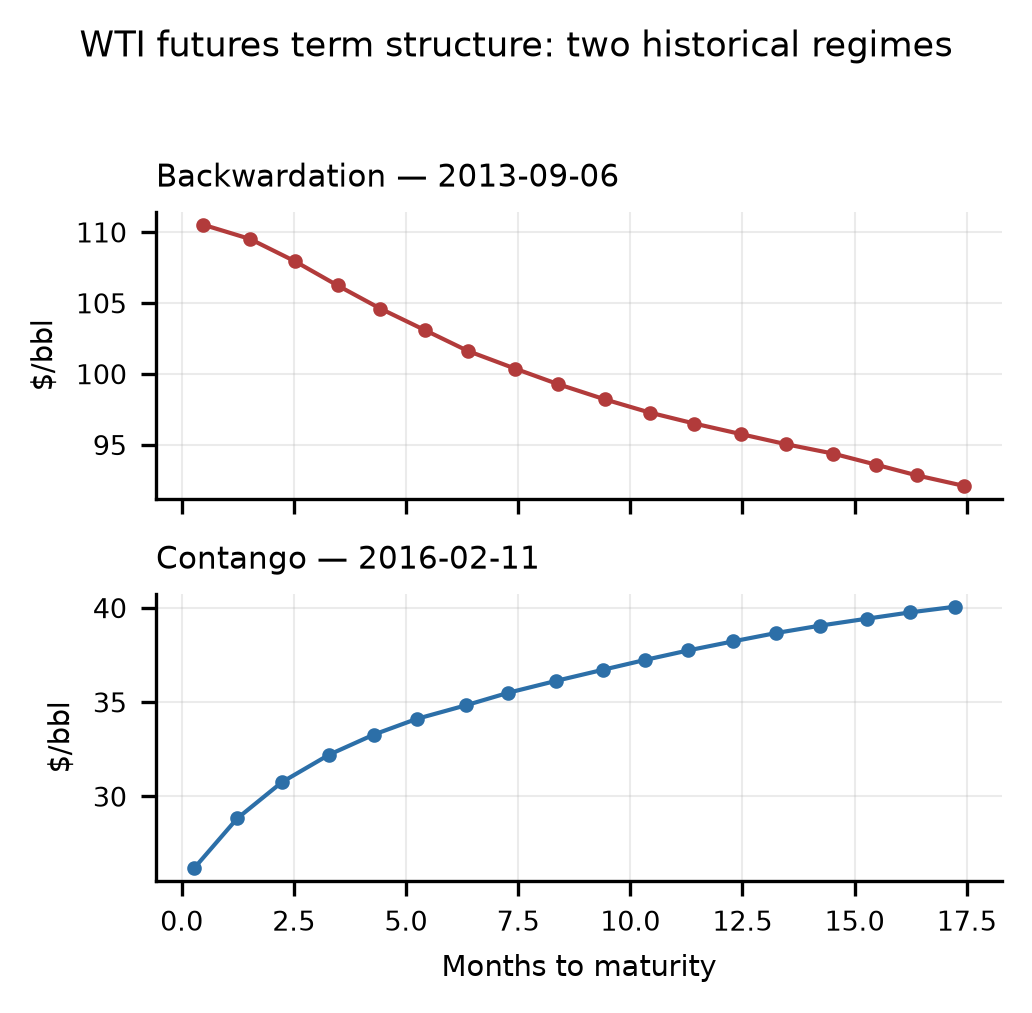
\includegraphics[width=\linewidth]{figs/Figure_1.png}
  \vspace{-6pt}
  \caption{Observed WTI futures term structures on two dates from the panel of Section~\ref{sec:data} (NYMEX settlement prices, 2010\rng{}2022). Left: 6~September~2013 (backwardation), showing short-maturity contracts trading above longer-dated ones. Right: 11~February~2016 (contango), during the 2014\rng{}2016 supply glut. Both panels plot the full eighteen-contract curve actually fitted throughout the paper, rather than a schematic.}
  \label{fig:term-structure-contango-backwardation}
  \vspace{-10pt}
\end{figure}

\subsection{Stylised empirical features}

Oil futures prices exhibit volatility clustering, heteroskedasticity, and structural breaks around macroeconomic and geopolitical shocks \cite{Pindyck1999, Du2025, Li2023}. Correlations across maturities are high but not perfect, which implies more than one source of uncertainty driving the curve \cite{SchwartzSmith2000, Kearney2019}. Taken together with the instability of the slope, these facts are what rule out single-factor specifications and motivate the framework developed in Section~\ref{sec:twofactor}. Figure~\ref{fig:garch_oil_volatility} shows the clustering and time-varying variance directly.

\begin{figure}[t]
  \centering
  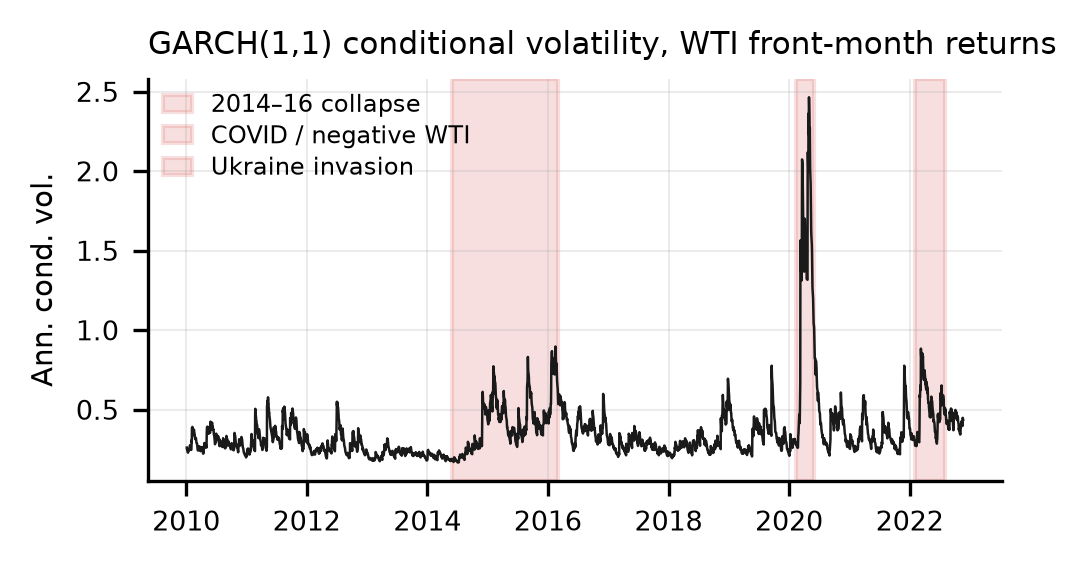
\includegraphics[width=\linewidth]{figs/figure_2.png}
\caption{Conditional volatility of WTI front-month log returns, GARCH(1,1) with Student-$t$ innovations fitted on the 2010\rng{}2022 panel of Section~\ref{sec:data} ($\hat\alpha=0.10$, $\hat\beta=0.89$, $\hat\nu=6.0$). Shaded regions mark the 2014\rng{}16 price collapse, the April 2020 COVID/negative-price episode, and the 2022 Russian invasion of Ukraine, illustrating volatility clustering and the structural breaks these episodes impose on oil price dynamics.}
\label{fig:garch_oil_volatility}
\end{figure}

\section{From Single-Factor to Multi-Factor Models}
\label{sec:models}

\subsection{Limitations of single-factor specifications}

Early commodity pricing models relied on a single stochastic driver, typically geometric Brownian motion or a mean-reverting process \cite{GibsonSchwartz1990, Pindyck1999}:
%
\begin{equation}
  dS_t = \mu S_t\,dt + \sigma S_t\,dW_t ,
\end{equation}
%
or, in mean-reverting form,
%
\begin{equation}
  dX_t = \kappa(\mu - X_t)\,dt + \sigma\,dW_t .
\end{equation}
%
Both are analytically convenient, however both fail on the term structure. With one state variable every maturity is a deterministic function of a single number, so the model cannot generate the imperfect cross-maturity correlations documented above, and cannot represent temporary price correction and structural shifts in the equilibrium anchor as separate phenomena \cite{SchwartzSmith2000, Pindyck1999}. The move to multiple factors is therefore substantive rather than cosmetic: it encodes the position that the long-run level is itself stochastic, responding to production capacity, technology, and macroeconomic conditions \cite{CasassusCollinDufresne2005, Ballestra2025}.

\subsection{Multi-factor frameworks}

Multi-factor models represent prices as a function of several latent state variables,

\begin{equation}
  S_t = f(X_{1,t}, X_{2,t}, \dots, X_{n,t}) ,
\end{equation}

each capturing a distinct economic influence. Because these drivers are unobservable, they must be recovered from the cross-section of contract maturities by filtering \cite{SchwartzSmith2000, Peters2011}. The added flexibility is well documented: Casassus and Collin-Dufresne show that stochastic convenience yield dynamics explain a meaningful part of the cross-section of futures prices while permitting time-varying risk premia across maturities \cite{CasassusCollinDufresne2005, HamiltonWu2014}.

The cost is estimation difficulty. Latent-variable estimates are sensitive to noise, to model specification, and to structural change, so performance depends on whether the mapping from prices to underlying conditions is stable over the sample \cite{Peters2011, Ballestra2025, SchwartzSmith2000}. Section~\ref{sec:identification} treats these difficulties concretely rather than as a general caveat.

\section{The Two-Factor Model and the Futures Curve}
\label{sec:twofactor}

\subsection{Specification}

Let $S_t$ denote the spot price of crude oil. Following the short-run/long-run decomposition, the log spot price is the sum of a transient and a persistent component,

\begin{equation}
  \ln S_t = \chi_t + \xi_t ,
  \label{eq:decomposition}
\end{equation}

where $\chi_t$ captures short-lived deviations that dissipate as inventories and logistics adjust, and $\xi_t$ represents the slower-moving equilibrium level toward which the market is understood to gravitate. Under the physical measure $\mathbb{P}$ the two factors evolve as

\begin{align}
  d\chi_t &= -\kappa\,\chi_t\,dt + \sigma_\chi\,dW^\chi_t ,
  \label{eq:chi_p} \\[2pt]
  d\xi_t  &= \mu_\xi\,dt + \sigma_\xi\,dW^\xi_t ,
  \label{eq:xi_p}
\end{align}
%
with $dW^\chi_t\,dW^\xi_t = \rho\,dt$ and $\kappa > 0$. The short-run factor is an Ornstein-Uhlenbeck process reverting to zero, so that $\ln S_t \to \xi_t$ in expectation; the long-run factor is an arithmetic Brownian motion, encoding the view that the equilibrium level is itself stochastic rather than a fixed anchor.

The economic content of \eqref{eq:chi_p}~\eqref{eq:xi_p} is the separation of horizons. A refinery outage or an inventory surprise perturbs $\chi_t$ and decays at rate $\kappa$; a structural shift in production capacity or in the trajectory of global demand moves $\xi_t$ and never decays. The half-life $\ln 2 / \kappa$ is therefore the model's central economic read-out, and a credible estimate should land in weeks to months rather than days or years.

\subsection{Risk-neutral dynamics}

Futures prices are expectations under the risk-neutral measure $\mathbb{Q}$, not under $\mathbb{P}$. Introducing a constant market price of risk for each factor gives
%
\begin{align}
  d\chi_t &= (-\kappa\,\chi_t - \lambda_\chi)\,dt + \sigma_\chi\,dW^{\chi,\mathbb{Q}}_t ,
  \label{eq:chi_q} \\[2pt]
  d\xi_t  &= \mu_\xi^{*}\,dt + \sigma_\xi\,dW^{\xi,\mathbb{Q}}_t ,
  \label{eq:xi_q}
\end{align}
%
where $\lambda_\chi$ is the short-run risk premium and $\mu_\xi^{*} = \mu_\xi - \lambda_\xi$ is the risk-neutral long-run drift. The distinction matters for interpretation: the wedge between $\mu_\xi$ and $\mu_\xi^{*}$ is precisely the compensation investors demand for bearing long-horizon oil price risk, which is the quantity that empirical work on oil risk premia seeks to measure \cite{HamiltonWu2014, Cortazar2022}.

\subsection{Closed-form futures price}

Because \eqref{eq:chi_q}\rng{}\eqref{eq:xi_q} is a linear Gaussian system, the futures price $F(t,T) = \mathbb{E}^{\mathbb{Q}}_t[S_T]$ admits a closed form. Writing $\tau = T - t$ for time to maturity,
%
\begin{equation}
  \ln F(t,T) = e^{-\kappa\tau}\chi_t + \xi_t + A(\tau) ,
  \label{eq:futures}
\end{equation}
%
with the deterministic adjustment
%
\begin{equation}
  \begin{aligned}
    A(\tau) = {}& \mu_\xi^{*}\tau
      - \bigl(1 - e^{-\kappa\tau}\bigr)\frac{\lambda_\chi}{\kappa} \\
      &+ \frac{1}{2}\Biggl[
          \bigl(1 - e^{-2\kappa\tau}\bigr)\frac{\sigma_\chi^{2}}{2\kappa}
          + \sigma_\xi^{2}\tau \\
      &\hspace{2.2em}
          + \,2\bigl(1 - e^{-\kappa\tau}\bigr)
            \frac{\rho\,\sigma_\chi\sigma_\xi}{\kappa}
        \Biggr] .
  \end{aligned}
  \label{eq:Atau}
\end{equation}
%
Equation \eqref{eq:futures} is the pivot of the entire framework, and its structure repays attention. The long-run factor enters every maturity with a loading of exactly one: a shock to $\xi_t$ shifts the whole curve in parallel. The short-run factor enters with loading $e^{-\kappa\tau}$, which decays in maturity: a shock to $\chi_t$ moves the front of the curve substantially and the deferred contracts barely at all. The two factors are thus not merely statistically distinct but \emph{observationally} distinct, and it is this cross-sectional separation that makes them recoverable from a panel of futures prices at all.

\subsection{Curve shape as a statement about the short-run factor}
\label{sec:slope}

The contango and backwardation regimes discussed in Section~\ref{sec:markets} follow directly from \eqref{eq:futures}. Differentiating with respect to maturity,
%
\begin{equation}
  \frac{\partial \ln F(t,T)}{\partial \tau}
    = -\kappa\, e^{-\kappa\tau}\chi_t + A'(\tau) ,
  \label{eq:slope}
\end{equation}
%
and evaluating at the front of the curve gives
%
\begin{equation}
  \begin{aligned}
    \left.\frac{\partial \ln F}{\partial \tau}\right|_{\tau=0}
      &= -\kappa\,\chi_t + \bar{a} , \\[2pt]
    \bar{a} &\equiv \mu_\xi^{*} - \lambda_\chi
      + \tfrac{1}{2}\bigl(\sigma_\chi^{2} + \sigma_\xi^{2}
        + 2\rho\,\sigma_\chi\sigma_\xi\bigr) ,
  \end{aligned}
  \label{eq:frontslope}
\end{equation}
%
where $\bar{a}$ is constant in $t$. The time-varying part of the front-end slope is driven entirely by $\chi_t$. The market is in backwardation when the short-run factor is sufficiently positive, that is, when the spot price sits above its equilibrium level, which is exactly the condition of physical tightness that the convenience-yield literature describes \cite{GibsonSchwartz1990, KilianMurphy2014}. Rather than simply accommodating contango and backwardation as empirical stylised facts, the framework endogenously derives them via a latent state variable. This provides a transparent economic sanity check for Section~\ref{sec:empirical}, where the filtered state $\hat{\chi}_t$ should track observed regime shifts by cleanly changing signs.

\subsection{Relation to Gabillon's formulation}
\label{sec:gabillon-relation}

Gabillon \cite{Gabillon1992} specifies the two state variables as the spot price and a stochastic long-term price $L_t$, with the spot reverting toward $L_t$ rather than toward a constant. Setting $X_t = \ln S_t$ and $\mu_t = \ln L_t$ yields
%
\begin{equation}
  dX_t = \kappa(\mu_t - X_t)\,dt + \sigma\,dW_t ,
  \qquad
  d\mu_t = \sigma_L\,dZ_t ,
  \label{eq:gabillon}
\end{equation}
%
which is a reparametrisation of \eqref{eq:chi_p}~\eqref{eq:xi_p} under the change of variables $\chi_t = X_t - \mu_t$, $\xi_t = \mu_t$. The two specifications are observationally equivalent up to the drift term in \eqref{eq:xi_p}, which \eqref{eq:gabillon} suppresses. This paper works in the $(\chi, \xi)$ parametrisation throughout, because it renders the loadings in \eqref{eq:futures} explicit and maps directly onto the state-space form developed next.

\subsection{Economic interpretation of the factors}

The short-run factor absorbs temporary deviations arising from market frictions, inventory imbalances, and informational shocks. These are closely related to movements in the convenience yield, since inventory levels govern the marginal value of immediate delivery \cite{GibsonSchwartz1990, KilianMurphy2014}, and stochastic convenience yield dynamics are known to contribute materially to the cross-section of futures prices \cite{CasassusCollinDufresne2005}.

The long-run factor reflects expectations about future supply-demand balance, technological development, and macroeconomic trends in energy markets \cite{Pindyck1999}. Structural changes in production capacity and consumption patterns shift the equilibrium level gradually, and the evidence that longer-maturity contracts embed compensation for systematic risk indicates that these expectations are priced rather than incidental \cite{HamiltonWu2014}.

\subsection{Extension to two mean-reverting factors}
\label{sec:threefactor}

The specification above assigns a single decay rate to every transient shock. That is a strong restriction, and Section~\ref{sec:kappaslide} reports the evidence that it fails on a panel of realistic depth: fitted on maturities out to eighteen months, $\kappa$ moves systematically with \emph{which} segment of the curve is included, because one exponential cannot simultaneously match the curvature at the front and the flatness at the back. The extension is therefore reported here rather than deferred, since the empirical sections use it throughout.

Let the transient component be the sum of two Ornstein-Uhlenbeck processes with distinct rates,
%
\begin{equation}
  \ln S_t = \chi_{1,t} + \chi_{2,t} + \xi_t ,
  \qquad
  \kappa_1 > \kappa_2 > 0 ,
  \label{eq:decomposition3}
\end{equation}
%
with $d\chi_{j,t} = -\kappa_j \chi_{j,t}\,dt + \sigma_j\,dW^j_t$ and a full correlation structure across the three innovations. The futures price retains its closed form,
%
\begin{equation}
  \ln F(t,T) = e^{-\kappa_1\tau}\chi_{1,t} + e^{-\kappa_2\tau}\chi_{2,t} + \xi_t + A(\tau) ,
  \label{eq:futures3}
\end{equation}
%
and $A(\tau)$ generalises term for term, the variance component acquiring a cross-factor entry in $\bigl(1-e^{-(\kappa_1+\kappa_2)\tau}\bigr)/(\kappa_1+\kappa_2)$. Setting $\sigma_2 = 0$ recovers \eqref{eq:futures} exactly, which is asserted numerically rather than by inspection.

Two identification points govern estimation and both are silent failures if neglected. The two transient factors are \emph{exchangeable}: without an ordering restriction an optimiser may swap them between starting values, and a multi-start diagnostic then reports spurious multi-modality that is only label switching. Estimation therefore parameterises $\kappa_1 = \kappa_2 + e^{g}$. Separately, under the null $\sigma_2 = 0$ the parameters $\kappa_2$ and $\lambda_2$ are unidentified, so the likelihood-ratio statistic for adding the factor does \emph{not} have a $\chi^2$ null: this is a boundary problem with unidentified nuisance parameters \cite{Davies1987}. Section~\ref{sec:threefit} accordingly evaluates the extension out of sample rather than by a nested test.

\section{Latent Factor Estimation as a State-Space Problem}
\label{sec:statespace}

\subsection{From pricing formula to estimable model}

Neither $\chi_t$ nor $\xi_t$ is observable. What is observable is a panel of futures settlement prices across $m$ maturities, and \eqref{eq:futures} is linear in the latent state. The estimation problem is therefore a linear Gaussian state-space model, for which the Kalman filter delivers both the factor estimates and the exact likelihood in a single pass.

Collect the state as $\bm{x}_t = (\chi_t, \xi_t)^{\!\top}$ and observe log futures prices $\bm{y}_t \in \mathbb{R}^{m}$ at maturities $\tau_{t,1},\dots,\tau_{t,m}$. Discretising \eqref{eq:chi_p}\rng{}\eqref{eq:xi_p} exactly over a step $\Delta t$ gives the transition equation
%
\begin{equation}
  \bm{x}_t = \bm{c} + \bm{T}\bm{x}_{t-1} + \bm{w}_t ,
  \qquad \bm{w}_t \sim N(\bm{0}, \bm{Q}) ,
  \label{eq:transition}
\end{equation}
%
with
%
\begin{equation}
  \bm{T} = \begin{pmatrix} e^{-\kappa\Delta t} & 0 \\ 0 & 1 \end{pmatrix} ,
  \qquad
  \bm{c} = \begin{pmatrix} 0 \\ \mu_\xi \Delta t \end{pmatrix} ,
\end{equation}
%
and $\bm{Q}$ symmetric with entries
%
\begin{equation}
  \begin{aligned}
    Q_{11} &= \bigl(1 - e^{-2\kappa\Delta t}\bigr)
              \frac{\sigma_\chi^{2}}{2\kappa} , \\[2pt]
    Q_{22} &= \sigma_\xi^{2}\,\Delta t , \\[2pt]
    Q_{12} = Q_{21} &= \bigl(1 - e^{-\kappa\Delta t}\bigr)
              \frac{\rho\,\sigma_\chi\sigma_\xi}{\kappa} .
  \end{aligned}
\end{equation}
%
The measurement equation follows from \eqref{eq:futures},
%
\begin{equation}
  \bm{y}_t = \bm{d}_t + \bm{Z}_t\bm{x}_t + \bm{v}_t ,
  \qquad \bm{v}_t \sim N(\bm{0}, \bm{H}) ,
  \label{eq:measurement}
\end{equation}
%
where row $i$ of $\bm{Z}_t$ is $\bigl(e^{-\kappa\tau_{t,i}},\; 1\bigr)$, $d_{t,i} = A(\tau_{t,i})$, and $\bm{H} = \operatorname{diag}(s_1^{2},\dots,s_m^{2})$. Figure~\ref{fig:state_space_gabillon} summarises the resulting structure.

Two features of \eqref{eq:measurement} deserve emphasis because they are routinely mishandled. First, $\bm{Z}_t$ and $\bm{d}_t$ are genuinely time-varying: time to maturity shrinks each trading day between roll dates, so treating the loadings as constant introduces a systematic error that grows across the roll cycle. Second, the measurement errors are not a nuisance appended for convenience. With two factors, any two contracts price exactly; observing $m > 2$ maturities over-identifies the state, and without $\bm{v}_t$ the system would be stochastically singular. The variances $s_i^2$ absorb bid-ask effects, non-synchronous settlement and model misspecification, and allowing them to differ across the curve matters because deferred contracts are materially less liquid than the front months.

\begin{figure}[H]
\centering
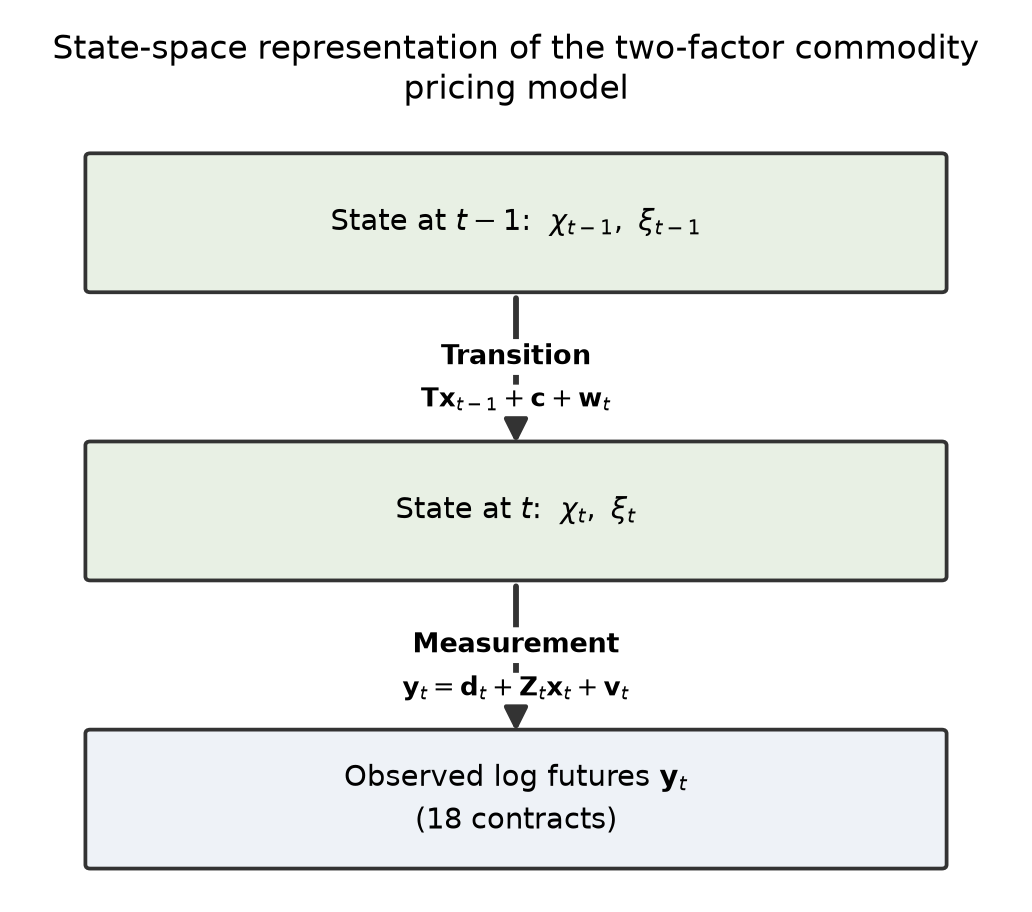
\includegraphics[width=\columnwidth]{figs/Figure_4.png}
\caption{State-space representation of the two-factor commodity pricing model. The short-run latent factor $\chi_t$ captures temporary deviations from equilibrium, while the long-run factor $\xi_t$ represents persistent structural expectations regarding supply-demand fundamentals. These latent states evolve according to the stochastic transition equation \eqref{eq:transition} and are linked to observed futures prices across maturities through the measurement equation \eqref{eq:measurement}.}
\label{fig:state_space_gabillon}
\end{figure}

\subsection{Likelihood and estimation}

Let $\bm{\theta} = (\kappa, \sigma_\chi, \sigma_\xi, \rho, \mu_\xi, \mu_\xi^{*}, \lambda_\chi, s_1,\dots,s_m)$. Running the filter yields one-step-ahead prediction errors $\bm{\nu}_t$ with covariance $\bm{S}_t$, and the prediction-error decomposition gives the exact log-likelihood
%
\begin{equation}
  \ell(\bm{\theta}) = -\frac{1}{2}\sum_{t=1}^{n}
    \Bigl[
      m_t\log 2\pi + \log\lvert\bm{S}_t\rvert
      + \bm{\nu}_t^{\!\top}\bm{S}_t^{-1}\bm{\nu}_t
    \Bigr] ,
  \label{eq:loglik}
\end{equation}
%
maximised numerically over $\bm{\theta}$. Here $m_t$ is the number of contracts actually observed at $t$, which handles the ragged panel exactly rather than by interpolation.

\subsection{Identification and practical difficulties}
\label{sec:identification}

Three issues bear directly on how results should be read, and stating them plainly is preferable to discovering them in the estimates.

\emph{The physical long-run drift is weakly identified.} Futures prices are $\mathbb{Q}$-expectations, so the panel pins down $\mu_\xi^{*}$ but carries little information about $\mu_\xi$. Estimates of $\mu_\xi$ from futures alone will carry wide standard errors. This is a structural feature of the model, not a numerical failure, and it should be reported rather than concealed by fixing the parameter silently.

\emph{The likelihood is multi-modal.} The pair $(\kappa, \sigma_\chi)$ trades off against the measurement-error variances: a fast-reverting, high-volatility short-run factor and a slow one with larger pricing errors can produce similar fits. Single-start optimisation is unreliable, and multi-start estimation with dispersed initial values is necessary rather than merely prudent.

\emph{Parameter stability is itself an empirical question.} Structural change in oil markets means $\bm{\theta}$ estimated on one decade need not apply to the next \cite{Pindyck1999, HamiltonWu2014, Cortazar2022}. Rolling-window re-estimation is treated in Section~\ref{sec:empirical} as a diagnostic, not only as a forecasting device.

% =====================================================================
\section{News as an Information Source}
\label{sec:news}
% =====================================================================

\subsection{Why news should matter here}

Expectations in commodity markets respond to geopolitical developments, macroeconomic conditions, and production decisions \cite{KilianMurphy2014, Pindyck1999}. Because such information is transmitted through financial news, policy statements and industry reports, textual data plausibly carries signal about supply disruptions, policy shifts and demand conditions, the same quantities that determine term structure dynamics \cite{HamiltonWu2014, Cortazar2022}.

The argument for this paper's specification is sharper than a general appeal to information content. Section~\ref{sec:twofactor} established that the two factors have distinct economic meanings and distinct maturity loadings. If news about immediate supply disruption moves $\chi_t$ while news about structural demand moves $\xi_t$, then text is not simply another predictor of returns: it is a source of information about \emph{which} factor is moving, and factor attribution is exactly what the filter finds hardest when prices alone are noisy.

\subsection{What the empirical literature has established}

Table~\ref{tab:news_studies} summarises the principal studies. Three patterns are worth drawing out, and one gap.

First, the evidence for incremental predictive content is reasonably consistent across text sources and methods. Gong, Guan and Chen find that textual features improve oil futures forecasting relative to price-only benchmarks \cite{Gong2022}; Pan, Wang and Yang report the same for futures returns using news-derived measures \cite{Pan2024}; Li et al.\ document gains for both returns and volatility using a decomposition-based deep learning design \cite{Li2021Sentiment}.

Second, the more careful studies find that raw sentiment polarity is not the right feature. Kaplan and co-authors show that hybrid models integrating economic theory and domain knowledge outperform generic sentiment classifiers \cite{Kaplan2023, Kaplan2024}, and Dai et al.\ argue explicitly for multi-dimensional signals over a single polarity score \cite{Dai2026}. Lexicon-based approaches tailored to the oil market show similar gains \cite{Li2025}. This informs the feature set in Section~\ref{sec:features}: net polarity alone is unlikely to be sufficient.

Third, methodological quality is uneven. A systematic review of news sentiment for asset price prediction notes recurring weaknesses in out-of-sample discipline and benchmark selection across this literature \cite{Ehsan2025}. Reported improvements are frequently in-sample, and the random walk is not always the comparison.

\emph{The gap.} Almost all of this work targets returns or realised volatility at a single horizon, typically the front contract. The \emph{term structure} is a markedly less common target, and the specific channel pursued here (text entering the latent state variables of an arbitrage-consistent pricing model, rather than entering a reduced-form predictor of returns) appears to be largely unexplored. Adjacent work applies machine learning to commodity factor discovery, but does so without imposing a pricing structure on the recovered factors \cite{Gupta2025}. Positioning the contribution this way is deliberate: the claim is that the channel is under-explored and worth testing, which the design in Section~\ref{sec:empirical} can substantiate, rather than a claim of outright priority, which a literature search cannot establish.

\subsection{Text representation}
\label{sec:features}

Machine learning methods differ in how they encode semantic, thematic and temporal structure, converting news into sentiment indicators, contextual embeddings, topic measures or lower-dimensional latent representations \cite{Gong2022, Pan2024, Li2023LLMFinance}. Appendix~\ref{app:ml_models} compares the principal architectures.

The specification adopted here follows the second pattern above and uses features aligned with the model's economic structure rather than a single polarity score: net sentiment, cross-sectional dispersion of sentiment, article volume, and topic shares over supply disruption, OPEC policy, geopolitics and demand conditions. Hybrid constructions combining text-derived measures with economically motivated variables provide the flexibility to attach different features to different factors \cite{Gong2022, Li2023}.

\subsection{The role of machine learning in this design}

The contribution of machine learning here is measurement, not replacement. Text-derived features are incorporated into a state-space representation that retains the arbitrage-consistent pricing structure of \eqref{eq:futures}, so the economic interpretation of the factors survives \cite{Peters2011, CasassusCollinDufresne2005}. This is deliberate. A flexible predictor trained directly on futures returns may forecast well and still say nothing about why; embedding text inside the factor dynamics keeps the estimated effects interpretable as statements about short-run deviation and long-run equilibrium. Figure~\ref{fig:news_augmented_framework} sets out the resulting architecture.

\begin{figure}[H]
\centering
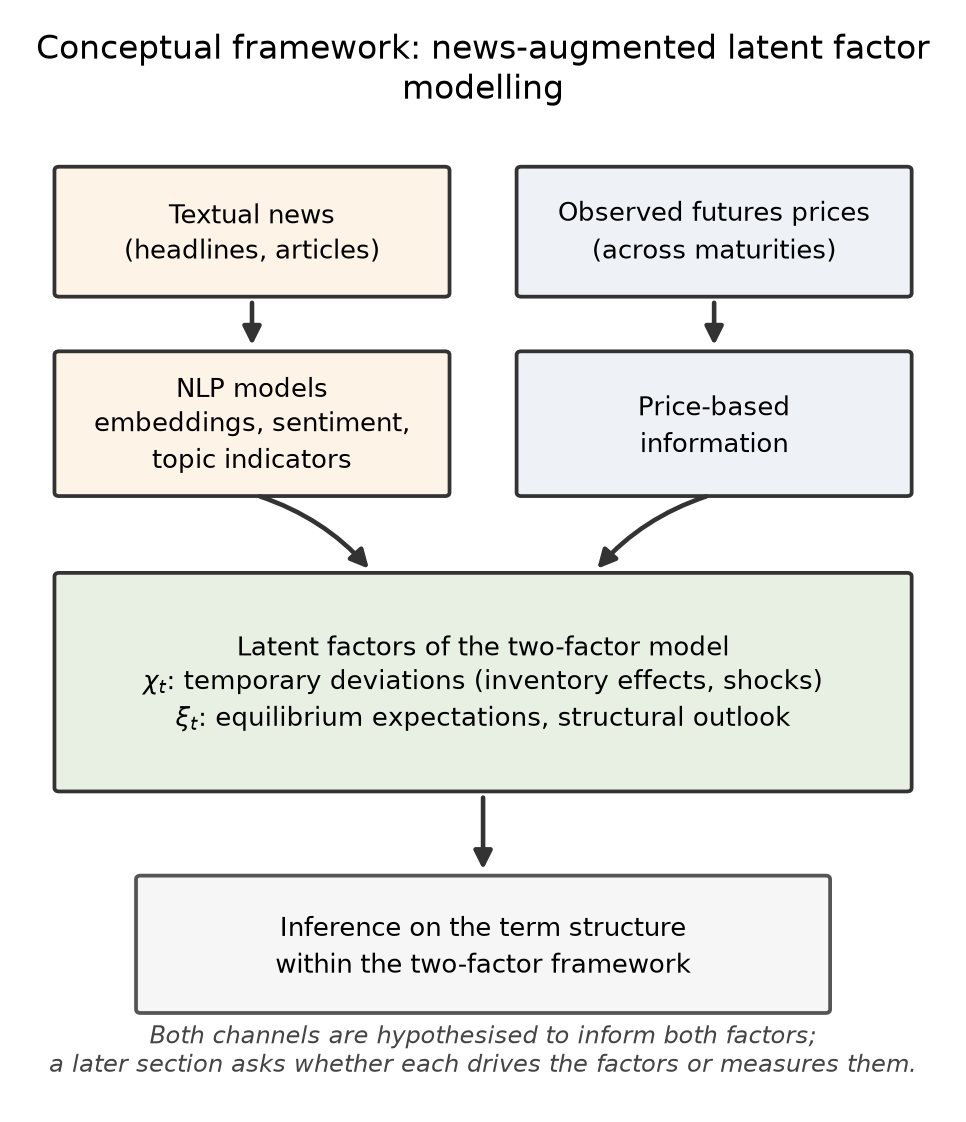
\includegraphics[width=\columnwidth]{figs/Figure_3.png}
\caption{Conceptual framework for news-augmented latent factor oil futures modelling. Textual news is processed using NLP models to extract embeddings, sentiment scores and topic indicators. These text-derived features inform the long-run factor, capturing equilibrium expectations and structural outlook, and the short-run factor, capturing temporary deviations driven by inventory effects and shocks. In parallel, observed futures prices across maturities provide price-based information. Both sources contribute to inference on the term structure within the two-factor framework.}
\label{fig:news_augmented_framework}
\end{figure}

% =====================================================================
\section{Empirical Design}
\label{sec:empirical}
% =====================================================================

The framework above yields a baseline against which the central claim of this paper can be tested. This section states the mechanism by which news enters the model, the hypotheses that follow, and the procedure used to evaluate them.

\subsection{How news enters the model}

The loose formulation that news sentiment ``improves estimation'' is not testable as stated. Making it testable requires specifying where in \eqref{eq:transition}\rng{}\eqref{eq:measurement} textual information acts. Two channels are considered, each nesting the baseline as a parameter restriction.

\emph{Channel A: sentiment as a driver of factor dynamics.} Let $\bm{u}_t \in \mathbb{R}^{p}$ collect the daily news features of Section~\ref{sec:features}. The transition equation \eqref{eq:transition} becomes
%
\begin{equation}
  \bm{x}_t = \bm{c} + \bm{T}\bm{x}_{t-1} + \bm{B}\bm{u}_{t-1} + \bm{w}_t ,
  \label{eq:channelA}
\end{equation}
%
with $\bm{B} \in \mathbb{R}^{2\times p}$. This formalises the economic claim that news revises expectations: sentiment relating to supply disruption should load on $\chi_t$, while sentiment relating to structural demand or production capacity should load on $\xi_t$. The lag on $\bm{u}_{t-1}$ is deliberate and enforced throughout, so that no signal is used before it could have been traded.

\emph{Channel B: news intensity as time-varying uncertainty.} Let $I_t$ denote standardised news volume. The short-run diffusion becomes
%
\begin{equation}
  \sigma_{\chi,t}^{2} = \sigma_\chi^{2}\exp(\gamma I_t) ,
  \label{eq:channelB}
\end{equation}
%
entering $\bm{Q}_t$ in place of $\bm{Q}$. The economic content is that on days of intense news flow the short-run factor is genuinely more volatile, and the filter should weight the prior less heavily against incoming prices.

\subsection{Hypotheses}

\begin{description}
  \item[H1] \textit{(Channel A)} $\bm{B} \neq \bm{0}$. News features carry information about the evolution of the latent factors beyond that already contained in the futures panel.
  \item[H2] \textit{(Channel B)} $\gamma \neq 0$. News intensity is informative about the conditional volatility of the short-run factor.
  \item[H3] \textit{(Out-of-sample)} The augmented model produces lower out-of-sample forecast error for the futures curve than both the baseline two-factor model and a random walk in futures prices.
\end{description}

H3 is the demanding one and is stated deliberately against the random walk. In-sample likelihood improvements are cheap; a term-structure model that cannot outperform ``tomorrow's curve equals today's curve'' has not demonstrated economic content.

\emph{All three are answered in Part~II, two of them entirely in the negative and the third in two halves.} H1 is rejected in Section~\ref{sec:newsresult}: the driver channel is not significant at any conventional level. H2 is rejected in Section~\ref{sec:h2result}, at a pre-test that makes fitting it unnecessary. H3 as stated is rejected in Section~\ref{sec:denoisetest}, on levels, spreads and butterflies, under both restricted and unrestricted factor dynamics, but that test is shown there to be a joint test of the measurement model and the transition, so it does not isolate the premise it was written for. Section~\ref{sec:h3a} separates the two: the cross-sectional claim is \emph{supported} on fourteen of eighteen maturities, and the temporal claim remains rejected. Each of the three was re-examined after rejection, on grounds stated in advance and independent of the outcome, and Sections~\ref{sec:h2result}, \ref{sec:h1prime} and~\ref{sec:h3a} report the originals alongside the revisions rather than in place of them.

The hedge that would ordinarily follow, namely that the informative result is the set of conditions under which the model succeeds, is not available here, and is not offered. There are no such conditions on this panel. What Part~II does report is a positive result on a channel this list does not contain, which is noted in the next paragraph rather than presented as a partial confirmation of these hypotheses.

\emph{A note on what Part~II adds.} The two channels above exhaust the ways news could enter the model \emph{as specified in Part~I}. Section~\ref{sec:driver-measurement} introduces a third on theoretical grounds (news as a second \emph{measurement} of the same latent shock rather than as a driver of it or a scaler of its variance), and Section~\ref{sec:lattice} commits it to the specification lattice before estimation. That channel is supported, at $p = 3.6\times10^{-7}$, and it is the paper's principal positive finding. It is reported as an addition to the pre-registered set rather than as one of its members, because it is one.

\subsection{Data}
\label{sec:data}

\emph{Futures.} Daily settlement prices for individual expiring NYMEX WTI contracts, assembled into a nearby-position panel by the exchange's own expiry rule: the third business day prior to the twenty-fifth calendar day of the month preceding delivery, on the NYMEX rather than the federal holiday calendar. The construction is deliberate: a panel built from a fixed month offset misdates the roll by up to thirty-two days, which propagates into $e^{-\kappa\tau}$ as a mean error of several percent in the loading that identifies $\kappa$.

The panel spans 6{,}516 trading days to twenty-four nearby positions, of which 2010\rng{}2022 is used. Coverage is 98 percent at position four, 93 at twelve and 89 at eighteen; missing cells are handled exactly by the filter rather than interpolated.

Provenance is verified rather than asserted. The source publishes open, high, low and close, and whether the close is the exchange's official settlement (a volume-weighted average over a defined window, not a last trade) is not documented. It is instead established against the U.S. Energy Information Administration's \texttt{RCLC1} series, which is an official settlement series: mapping the assembled panel onto nearby position one by the same expiry rule and differencing over 3{,}236 overlapping days gives exact agreement on \textbf{99.94 percent} of days, with every year from 2011 to 2022 matching on all sessions and only two days differing in the entire sample. A wedge between a close and a settlement would widen on volatile days; none is present. This is a stronger provenance argument than vendor documentation, and it costs nothing.

The sample ends in November 2022, which shortens the joint news/price window to 2015\rng{}2022, roughly 1{,}950 trading days. That is a property of the source rather than of the design, and it is recorded in Section~\ref{sec:risk}.

\emph{Text.} A daily corpus of oil-related news, scored with a finance-domain sentiment model \cite{Araci2019}. Documents are aggregated to daily frequency by publication timestamp and lagged one trading session. Features are as specified in Section~\ref{sec:features}.

\subsection{Testing procedure}

\emph{Estimator validation.} Before any inference on market data, the filter is applied to simulated panels generated from known parameters. Recovery of those parameters within their estimated standard errors is a precondition for interpreting anything that follows; this is reported first in Part~II.

\emph{In-sample.} H1 and H2 are nested restrictions, so both are tested by likelihood ratio, $2(\ell_{\text{aug}} - \ell_{\text{base}}) \sim \chi^2_q$, supported by AIC and BIC.

\emph{Out-of-sample.} Expanding-window re-estimation with forecasts of the full curve at horizons of one, five and twenty-two trading days. Forecast accuracy is compared by Diebold-Mariano test against both benchmarks.

\emph{Conditional performance.} Results are split by curve regime (contango versus backwardation, classified by the sign of the fitted front-end slope in \eqref{eq:frontslope}), by realised volatility tercile, and by news-intensity tercile. H3 is most plausible in high-intensity, regime-transition periods, and reporting the split is more informative than a single pooled statistic.

\emph{Economic evaluation.} Filtered factors imply a fitted curve; deviations of observed from fitted prices define calendar-spread signals. Performance is reported net of transaction costs, since a statistical edge that does not survive the bid/ask spread is not an edge.

\subsection{Threats to validity}

Three concerns are addressed explicitly rather than deferred to a limitations paragraph. \emph{Look-ahead bias:} publication timestamps are not tradeable timestamps, hence the enforced one-session lag. \emph{Pretraining contamination:} the sentiment model has seen financial text from the evaluation period during pretraining; this is acknowledged and probed with a lexicon-based sentiment measure as robustness \cite{Li2025}. \emph{Endogeneity:} news reports price movements as well as anticipating them, so $\bm{u}_t$ is not exogenous in the strict sense. A placebo specification with date-shuffled news features is estimated to establish that measured improvements are not an artefact of mechanical correlation with contemporaneous returns.

\section{Conclusion to Part I}

Part~I has developed a two-factor representation of the oil futures curve in which the closed-form pricing equation \eqref{eq:futures} maps onto a state-space model, making the latent factors recoverable by filtering and the parameters estimable by maximum likelihood. Two results are worth restating. The contango/backwardation distinction is not an additional stylised fact to be accommodated but a consequence of the model, with the front-end slope determined by the sign of the short-run factor. And the difficulty of latent factor estimation is specific and diagnosable (weak identification of the physical drift, a multi-modal likelihood, and parameter instability across regimes) rather than a general caveat.

Against that baseline, the question of whether news carries incremental information becomes a testable proposition. Sections~\ref{sec:news} and~\ref{sec:empirical} specified two channels, stated three hypotheses, and set out an evaluation protocol built around out-of-sample curve forecasting, regime-conditional reporting, and a placebo control. The design deliberately makes the claim easy to refute: the random-walk benchmark is hard to beat, and a date-shuffled news series should destroy any genuine effect.

Textual sentiment is a complementary information source, not a substitute for structural pricing models. News-derived features are noisy, potentially unstable over time, and vulnerable to distortion from low-quality reporting. Whether they add anything, and under what market conditions, is the subject of Part~II.

% =====================================================================
\section{Implementation Design}
\label{sec:implementation}

Part~II implements the framework developed in Part~I and evaluates its measurement and forecasting implications separately. The analysis first distinguishes news entering the transition equation from news entering the observation equation. It then validates the estimator on simulated data, examines specification failures on the WTI panel, and evaluates the incremental information in news.

\subsection{Prices and news as observation channels}
\label{sec:instrument}

The disturbances $\bm{v}_t$ in \eqref{eq:measurement} allow an overidentified futures panel to depart from the curve implied by the latent factors. They may reflect bid--ask effects, non-synchronous settlements, limited liquidity, or model misspecification. An estimated observation variance therefore measures unexplained variation under the fitted model; it is not, by itself, an estimate of physical settlement error.

This distinction motivates treating prices and news as separate observation channels for a common latent process. The Kalman filter combines their information according to the specified covariance structure. Whether that weighting improves estimation must be evaluated empirically rather than inferred from the filter's construction.

Two assessments are used below. Same-day pricing of excluded maturities tests cross-sectional information recovery (Section~\ref{sec:h3a}), while one-step-ahead forecasting tests the observation model and transition dynamics jointly (Section~\ref{sec:denoisetest}). The filter improves the former over much of the curve but underperforms the random walk in the latter, particularly near expiry. These findings limit the interpretation of the latent states without invalidating the distinction between the two news channels.

\subsection{Transition and measurement mechanisms}
\label{sec:driver-measurement}

News can enter the model through two distinct mechanisms. In the driver specification, lagged features enter the transition equation through $\bm{B}$ in \eqref{eq:channelA}. A non-zero loading indicates incremental association with the subsequent factor transition, conditional on the model's price information. It does not establish that publication causes the market to move.

In the measurement specification, news provides an additional observation of a latent innovation through $\bm{G}$. This channel asks whether text helps characterise a shock associated with the current observation window, rather than whether it predicts the next transition.

The encompassing specification includes both channels. Their restrictions permit separate tests of incremental fit, subject to a common observation set and satisfactory optimisation. Neither statistical association alone establishes a tradable signal or identifies a causal effect.

\subsection{Augmenting the state to expose innovations}
\label{sec:augment}

Daily news features summarise information flow. The measurement specification therefore links them to factor innovations rather than to accumulated factor levels. This is a modelling choice: text may also contain information about persistent levels, but that alternative is outside the fitted specification.

For the two-factor model, expose the current disturbances by augmenting the state:
\begin{equation}
  \bm{z}_t = \bigl(\chi_t,\ \xi_t,\ w^\chi_t,\ w^\xi_t\bigr)^{\!\top} ,
  \label{eq:augstate}
\end{equation}
The transition matrix is
\begin{equation}
  \bm{T}^{a} =
  \begin{pmatrix}
    e^{-\kappa\Delta t} & 0 & 0 & 0 \\
    0 & 1 & 0 & 0 \\
    0 & 0 & 0 & 0 \\
    0 & 0 & 0 & 0
  \end{pmatrix} ,
  \label{eq:augT}
\end{equation}
The zero lower block resets the exposed disturbances each period. Crucially, the disturbance entering the level block and its exposed counterpart must be the same random quantity. With $\bm{z}_t=(\bm{x}_t^{\!\top},\bm{w}_t^{\!\top})^{\!\top}$, the augmented process covariance is
\[
\bm{Q}^{a}=\begin{pmatrix}\bm{Q}&\bm{Q}\\\bm{Q}&\bm{Q}\end{pmatrix},
\]
with intercept $(\bm{c}^{\!\top},\bm{0}^{\!\top})^{\!\top}$. Treating the two disturbance blocks as independent would define a different model and sever the intended link between news and state innovations.

Prices load on factor levels,
\begin{equation}
  \bm{y}_t = \bm{d}_t + \bigl[\,\bm{Z}_t \,\big|\, \bm{0}\,\bigr]\bm{z}_t + \bm{v}_t ,
  \label{eq:priceblock}
\end{equation}
whereas news loads on the exposed innovations:
\begin{equation}
  \bm{n}_t = \bm{a}_n + \bigl[\,\bm{0} \,\big|\, \bm{G}\,\bigr]\bm{z}_{t-\Delta_\ell} + \bm{e}_t ,
  \qquad \bm{e}_t \sim N(\bm{0}, \bm{R}_t) ,
  \label{eq:newsblock}
\end{equation}
Here $\bm{G}\in\mathbb{R}^{p\times2}$, and $\Delta_\ell$ indexes the alignment described in Section~\ref{sec:leadlag}. For a correctly represented lag structure and Gaussian disturbances, the system remains linear Gaussian. Non-zero lags require retaining the relevant innovation history; the contemporaneous four-dimensional representation alone does not implement an arbitrary lag.

The fitted news specifications use the three-factor price model of Section~\ref{sec:threefactor}. Their augmented state is five-dimensional, $(\chi_{1,t},\chi_{2,t},\xi_t,w^{\chi_1}_t,w^{\chi_2}_t)^{\!\top}$. Both news channels act only on the two mean-reverting factors: $\bm{B}$ enters their transitions and $\bm{G}$ observes their innovations. Neither channel loads on the innovation to $\xi_t$. The empirical tests consequently concern transient and cyclical shocks, not the ability of news to explain permanent equilibrium shifts.

\subsection{Nested channel specifications}
\label{sec:lattice}

Table~\ref{tab:lattice} defines the four channel specifications. The measurement channel was introduced in Part~II, after the original Part~I hypotheses; fixing this comparison set before its estimation does not make it part of the original hypothesis set.
\begin{table}[H]
\centering
\caption{Channel specification lattice}
\label{tab:lattice}
\small
\renewcommand{\arraystretch}{1.2}
\begin{tabular}{@{}llp{3.1cm}@{}}
\toprule
\textbf{Spec} & \textbf{Restriction} & \textbf{Reading} \\
\midrule
$\mathrm{S0}$  & $\bm{B}=\bm{0},\ \bm{G}=\bm{0}$ & Baseline, prices only \\
$\mathrm{SD}$  & $\bm{G}=\bm{0}$                 & News drives the factors \\
$\mathrm{SM}$  & $\bm{B}=\bm{0}$                 & News measures the innovations \\
$\mathrm{SDM}$ & unrestricted                    & Both channels \\
\bottomrule
\end{tabular}
\end{table}

Likelihood-ratio comparisons require identical observations in every specification. For this purpose, the restricted baseline retains the news observation rows with zero shock loadings and a specified null news density. A genuinely price-only likelihood cannot be subtracted from a joint price--news likelihood. Table~\ref{tab:lattice} uses ``prices only'' to describe the state-information restriction, not permission to omit observations from the comparison.

Numerical checks require restricted specifications to reproduce the corresponding parent likelihood within $10^{-9}$. These checks validate implementation of the restrictions; they do not establish that the optimiser reaches the global maximum or that the likelihood-ratio statistic has its nominal asymptotic distribution. The optimisation limitation for $\mathrm{SDM}$ is reported in Section~\ref{sec:newsresult}.

\subsection{Intensity-dependent news variance}
\label{sec:Rt}

Daily net sentiment is averaged over the documents available in an observation window. Its precision can therefore vary with article count and within-window dispersion. The proposed plug-in covariance is
\begin{equation}
  \bm{R}_t = \frac{\varsigma_t^{2}}{\max(I_t,\,1)}\,\bm{\Omega} ,
  \label{eq:Rt}
\end{equation}
where $\varsigma_t^2$ denotes document-level sentiment dispersion and $\bm{\Omega}$ describes cross-feature dependence. The implementation sets $\bm{\Omega}=\bm{I}$ to retain diagonal observation covariance. Each feature is assigned the same scalar variance; cross-feature dependence is not estimated.

In this equation $I_t$ is the raw count after near-duplicate removal, distinct from the standardised intensity entering the process-variance equation. Standardised counts can be negative and cannot serve as a denominator. The $\max(I_t,1)$ convention avoids division by zero but does not create an observed sentiment value on a day with no documents; missing news observations require separate treatment.

The inverse-count scaling is an approximation that assumes limited dependence among retained documents. Common sources and correlated reporting can make the effective sample size smaller than the count. More coverage raises the news channel's precision under this specification, conditional on dispersion, but does not necessarily raise every element of the Kalman gain.

\subsection{Time-varying state and price-channel variance}
\label{sec:QH}

Time variation is allowed in both factor innovation variance and price observation variance. These components address different sources of uncertainty and should be distinguished from one another.

The proposed process-variance equation extends Channel~B:
\begin{equation}
  \sigma_{\chi,t}^{2}
    = \sigma_\chi^{2}\exp\!\bigl(\gamma I_t + \gamma_r \mathbb{1}_t^{\text{rel}}
      + \gamma_v \widehat{\mathrm{RV}}_{t-1}\bigr) ,
  \label{eq:Qt}
\end{equation}
The release indicator $\mathbb{1}_t^{\mathrm{rel}}$ represents scheduled information arrivals, and $\widehat{\mathrm{RV}}_{t-1}$ is lagged realised volatility. A scheduled date is predetermined, although the information released on that date need not be exogenous to market conditions. For forecasting, intensity and volatility inputs must be available when the state prediction is formed; contemporaneous inputs instead define a conditional nowcasting exercise.

Using lagged realised volatility avoids conditioning a forecast prior on the current prices it is intended to explain. With predetermined covariates, the Gaussian recursions remain valid conditional on those covariates. That statement does not extend automatically to the Student-$t$ and robust specifications in Section~\ref{sec:robust}.

Roll-related observation variance is represented by
\begin{equation}
  \bm{H}_t = \operatorname{diag}\!\bigl(s_i^{2}
    \exp(\eta \mathbb{1}_t^{\text{roll}})\bigr) ,
  \label{eq:Ht}
\end{equation}
where the front contract's exchange-calendar roll window supplies a curve-wide indicator. The implementation estimates one shared $\eta$, rather than a separate coefficient for each maturity. This is a parsimonious way to allow settlement uncertainty to change around rolls, not a direct estimate of each contract's liquidity.

The estimated roll effect can inform the conditional-news hypothesis H4, provided the observation variance has a credible interpretation. Section~\ref{sec:varid} assesses whether process- and observation-variance scalings can be distinguished in calibrated simulations; this does not establish identification under all market specifications.

\subsection{Asymmetric feature loadings}
\label{sec:asym}

Supply disruptions and demand weakness may have asymmetric effects because inventories face non-negativity and capacity constraints. The feature construction allows different responses to positive and negative observations:
\begin{equation}
  \bm{u}^{+}_t = \max(\bm{u}_t, \bm{0}), \qquad
  \bm{u}^{-}_t = \min(\bm{u}_t, \bm{0}) ,
  \label{eq:asym}
\end{equation}
The restriction $\bm{G}^{+}=\bm{G}^{-}$ defines symmetric loadings. The split is on observed features rather than on the unobserved innovation. Splitting on a latent sign would create a nonlinear observation map and require different filtering methods.

Observed-sign conditioning also needs care in the measurement channel. If a news observation determines its own loading, linearity conditional on that loading is insufficient to establish a properly normalised joint Gaussian likelihood. The asymmetric specification therefore requires an explicit conditional or piecewise observation density before exact-likelihood inference can be claimed. It is not used as evidence for the principal channel comparison reported below.

\subsection{Feature construction and collinearity}
\label{sec:collinear}

Multiple text features can produce poor conditioning. Topic shares are compositional and sum to one, making a full set exactly collinear with an intercept. One topic is therefore omitted as the reference category. The retained topic block is orthogonalised against sentiment to reduce residual collinearity; any such transformation used in forecasting must be estimated within the training sample.

The specifications used for likelihood-based inference are unpenalised. Penalisation changes the estimator and can invalidate the usual likelihood-ratio reference distribution, particularly when selection occurs at zero. Ridge regularisation is reserved for prediction-only comparisons and must be reported separately from the nested inferential specifications.

\subsection{Robustness to heavy tails}
\label{sec:robust}

Gaussian observation models can be sensitive to outliers in settlements and news features. Secondary specifications consider a Huber-type robust filter and a Student-$t$ observation density fitted by expectation--maximisation. The former limits the influence of large residuals; the latter estimates tail thickness through the degrees-of-freedom parameter.

These alternatives change the statistical model as well as the treatment of extreme observations. The Student-$t$ model is not an exact linear-Gaussian filter marginally, even if Gaussian recursions are used conditionally within a mixture or iterative approximation. Accordingly, \eqref{eq:loglik} is the exact likelihood of the Gaussian baseline, not automatically of every robust extension.

An unscented Kalman filter would address nonlinear transition or observation maps. It does not, by itself, correct heavy-tailed disturbances in the linear system used here.

\subsection{Lead/lag and timestamp diagnostics}
\label{sec:leadlag}

The offset $\Delta_\ell$ in \eqref{eq:newsblock} is examined over a lead--lag grid. Positive offsets associate a news observation with an earlier innovation and may indicate delayed reporting. Negative offsets associate it with a later innovation and warrant checks of timing conventions, daily aggregation and publication metadata. Neither sign alone diagnoses timestamp contamination: genuine predictive information and differing settlement windows can also affect the alignment.

Specifications used for prospective inference impose $\Delta_\ell\geq1$. With the indexing in \eqref{eq:newsblock}, news dated $t$ then measures an innovation no later than $t-1$. References below to a ``contemporaneous'' measurement should therefore be understood as an association within the aligned observation window, not evidence of an intraday causal ordering. Publication timestamps and exchange settlement times must provide the primary timing validation.

\subsection{State uncertainty as a sizing input}
\label{sec:sizing}

The filter provides a posterior covariance $\bm{P}_t$ as well as a state estimate. In a proposed trading evaluation, exposure can be scaled inversely with the posterior standard deviation of the signal-bearing factor. This scaling is meaningful only to the extent that the uncertainty estimates are calibrated.

To limit turnover, the proposed rebalancing rule is
\begin{equation}
  \bigl|\Delta\hat{\chi}_t\bigr| \;>\; \zeta\,\sqrt{P_{t,11}} \;+\; \tfrac{1}{2}\,\varkappa_t ,
  \label{eq:notrade}
\end{equation}
where $P_{t,11}$ is the short-run factor's posterior variance, $\varkappa_t$ is the round-trip spread cost in log-price units, and $\zeta$ controls the uncertainty threshold. The rule combines a statistical threshold with an execution-cost threshold. It is a practical approximation rather than a derived optimal policy under transaction costs.

The proposed protocol includes sensitivity to $\zeta$, a turnover cap and performance net of bid--ask costs. Study~C was not executed, so no sizing performance or economic benefit is claimed.

\section{Estimator Validation}
\label{sec:validation}

Validation begins with simulated panels whose parameters and latent states are known. These exercises test the estimator under controlled assumptions; they do not establish that the same assumptions hold for WTI. The market-data diagnostics that follow assess that separate question.

The baseline simulations use parameters close to the Schwartz--Smith crude oil estimates \cite{SchwartzSmith2000}, $n=2520$ daily observations and $m=4$ contracts with monthly rolls. Other exercises use the sample sizes stated in their tables.

\subsection{Parameter recovery}
\label{sec:recovery}

Table~\ref{tab:recovery} summarises 150 Monte Carlo replications. Mean biases are small relative to the Monte Carlo standard deviations. Empirical coverage of nominal 95\% intervals ranges from 0.920 to 0.973, broadly consistent with nominal coverage at this replication count, although several parameters show mild undercoverage.

Estimated standard errors are generally close to the Monte Carlo standard deviations. This supports their use in the simulated baseline, rather than establishing calibration for the misspecified or non-Gaussian market-data extensions.
\begin{table*}[!t]
\centering
\caption{Monte Carlo parameter recovery. 150 replications, $n=2520$, $m=4$. Coverage is the empirical frequency with which the nominal 95\% interval contains the true value.}
\label{tab:recovery}
\small
\renewcommand{\arraystretch}{1.15}
\begin{tabular}{@{}lrrrrrr@{}}
\toprule
\textbf{Parameter} & \textbf{True} & \textbf{Mean est.} & \textbf{Bias} & \textbf{MC s.d.} & \textbf{Mean s.e.} & \textbf{Coverage} \\
\midrule
$\kappa$        & 1.4900 & 1.5057 & $+0.0157$ & 0.0933 & 0.0832 & 0.927 \\
$\sigma_\chi$   & 0.2860 & 0.2843 & $-0.0017$ & 0.0144 & 0.0139 & 0.933 \\
$\sigma_\xi$    & 0.1450 & 0.1455 & $+0.0005$ & 0.0075 & 0.0067 & 0.920 \\
$\rho$          & 0.3000 & 0.3136 & $+0.0136$ & 0.0930 & 0.0889 & 0.933 \\
$\mu_\xi$       & 0.0000 & $-0.0061$ & $-0.0061$ & 0.0470 & 0.0458 & 0.947 \\
$\mu_\xi^{*}$   & 0.0115 & 0.0087 & $-0.0028$ & 0.0135 & 0.0123 & 0.920 \\
$\lambda_\chi$  & 0.1570 & 0.1529 & $-0.0041$ & 0.0854 & 0.0857 & 0.967 \\
$s_1$           & 0.0080 & 0.0080 & $<10^{-4}$ & 0.0001 & 0.0001 & 0.920 \\
$s_2$           & 0.0030 & 0.0030 & $<10^{-4}$ & 0.0001 & 0.0001 & 0.973 \\
$s_3$           & 0.0030 & 0.0030 & $<10^{-4}$ & 0.0001 & 0.0001 & 0.953 \\
$s_4$           & 0.0070 & 0.0070 & $<10^{-4}$ & 0.0001 & 0.0001 & 0.947 \\
\bottomrule
\end{tabular}
\end{table*}

\subsection{Identification revisited}
\label{sec:identification2}

The simulation supports the weak-precision concern for the physical drift $\mu_\xi$. Its mean estimate is $-0.0061$ when the true value is zero, and its interval coverage is 0.947. The mean standard error is approximately 0.046, so an annual drift of four percent would be difficult to distinguish from zero in this design.

Relative to their non-zero true values, the Monte Carlo standard deviations are particularly large for $\mu_\xi^{*}$ (ratio 1.18) and $\lambda_\chi$ (ratio 0.54). Diffusion and observation-variance parameters are more precisely recovered. The panel therefore identifies these components more accurately than the risk-premium quantities at the chosen calibration. Section~\ref{sec:kappa} examines how additional curve depth improves cross-sectional separation.

\subsection{Test size and power}
\label{sec:sizepower}

The Channel~A likelihood-ratio test is evaluated under the null and under one specified non-zero driver alternative (Table~\ref{tab:sizepower}). The empirical rejection rate is 0.033 under the null and 1.000 under that alternative.

With 60 replications, the binomial standard error at a nominal rejection probability of 0.05 is approximately 0.028. The null result is therefore compatible with nominal size. The observed power is high for the simulated effect, but does not establish sensitivity to smaller effects or to driver mechanisms excluded from the fitted model.
\begin{table}[H]
\centering
\caption{Size and power of the Channel~A likelihood-ratio test at the 5\% level, 60 replications each, $n = 1512$.}
\label{tab:sizepower}
\small
\renewcommand{\arraystretch}{1.2}
\begin{tabular}{@{}lcc@{}}
\toprule
\textbf{Data-generating process} & \textbf{Reject rate} & \textbf{Nominal} \\
\midrule
$\bm{B} = \bm{0}$ (size)     & 0.033 & 0.05 \\
$\bm{B} \neq \bm{0}$ (power) & 1.000 & n/a \\
\bottomrule
\end{tabular}
\end{table}

\subsection{Simulation-based identification of variance channels}
\label{sec:varid}

Both process noise and observation noise enter the prediction-error covariance, $\bm{S}_t=\bm{Z}_t\bm{P}_{t|t-1}\bm{Z}_t^{\!\top}+\bm{H}_t$. Joint estimation may therefore create a trade-off between their variance scalings.

The diagnostic simulates constant-variance panels and computes the observed information in $(\gamma_v,\eta)$ at the origin. Table~\ref{tab:varid} reports the implied estimate correlation and condition number under alternative driver configurations.
\begin{table}[H]
\centering
\caption{Identification of the process-noise and measurement-noise scalings. Simulated panels, $n = 1260$. Correlation is implied by the inverse observed information; a value near $\pm 1$ would indicate the two scalings are not separately identified.}
\label{tab:varid}
\small
\renewcommand{\arraystretch}{1.2}
\begin{tabular}{@{}lcc@{}}
\toprule
\textbf{Driver configuration} & \textbf{Corr.} & \textbf{Cond.\ no.} \\
\midrule
Identical driver on both channels & $-0.020$ & 5.6 \\
Volatility-like driver vs.\ roll calendar & $+0.007$ & 5.2 \\
Two independent drivers & $-0.002$ & 5.4 \\
\midrule
Identical driver, only $m = 2$ contracts & $-0.049$ & 2.1 \\
\bottomrule
\end{tabular}
\end{table}

The correlations are close to zero and the condition numbers are modest, including with identical drivers and only two contracts. At this calibration, the scalings are distinguishable because process noise propagates through shared factor loadings, whereas diagonal observation noise has a contract-specific cross-sectional pattern.

These results support joint estimation in the simulated setting. They do not remove the need to examine curvature, boundary behaviour and parameter stability in the fitted market model.

\subsection{Regime classification under known measurement noise}
\label{sec:denoise}

In a simulation with known latent prices, front-spread measurement error has a standard deviation equal to 62\% of the true spread's standard deviation. Table~\ref{tab:denoise} compares the observed price-ordering classifier with the filtered-state classifier against the noiseless regime.
\begin{table}[H]
\centering
\caption{Regime classification accuracy against the known true regime, $n = 3000$ simulated observations.}
\label{tab:denoise}
\small
\renewcommand{\arraystretch}{1.2}
\begin{tabular}{@{}lc@{}}
\toprule
\textbf{Classifier} & \textbf{Accuracy} \\
\midrule
Observed ordering, $F_1 > F_2$ & 0.843 \\
Filtered state, $\hat{\chi}_t$ via \eqref{eq:frontslope} & \textbf{0.974} \\
\bottomrule
\end{tabular}
\end{table}

Accuracy rises from 0.843 to 0.974. The result illustrates the potential benefit of combining noisy observations when the fitted model matches the data-generating process. It also motivates H4: an additional measurement channel may be more useful when price observations provide less precise state information.

The simulation does not justify replacing observed market regimes with filtered labels without further validation. WTI has no observed latent-state ground truth, and the fitted observation disturbance can contain persistent model error. Sections~\ref{sec:denoisetest} and~\ref{sec:h3a} therefore assess temporal forecasting and same-day pricing separately.

\subsection{A degenerate measurement-error profile}
\label{sec:firstcontact}

An eight-contract baseline with freely estimated diagonal observation covariance produces the following standard deviations, in basis points of log price:
\[
[320.2,\;162.1,\;52.9,\;16.2,\;1.4,\;5.5,\;1.4,\;10.0].
\]
The front-contract value corresponds to approximately \$2.24 at a \$70 price, while the fifth and seventh contracts reach the imposed one-tick floor. This profile is difficult to interpret as settlement uncertainty alone.

Removing the floor reduces those two entries to 0.0021 and 0.0233 basis points and raises the log-likelihood by 47. The two-factor fit thus approaches exact pricing of two selected contracts, resembling the exact-observation normalisation of Chen and Scott \cite{ChenScott1993}. The remaining contracts absorb discrepancies between the fitted curve and the panel.

This is an observed degeneracy in the fitted specification, not a general theorem that every likelihood increases whenever $k$ of $m$ observations are made exact. Its practical consequence is nevertheless clear: refitting overlapping contract subsets changes which maturities receive inflated variances. The free profile is insufficiently stable to support a structural interpretation. A proposed front-end storage explanation based on that profile was consequently not retained.

\subsection{A smooth measurement-error curve}
\label{sec:smoothcurve}

To restrict isolated near-zero variances, the free contract-specific standard deviations are replaced by a smooth maturity function:
\begin{equation}
  s(\tau) = \exp\bigl(a + b\,\tau + c\,\tau^{2}\bigr) ,
  \label{eq:smoothmeas}
\end{equation}
Adjacent maturities must then have related uncertainty levels. This excludes the alternating near-exact and high-error pattern observed in the free-diagonal fit, although variances can still approach zero near a panel endpoint.

The smooth form reduces the covariance parameter count and makes repeated panel diagnostics more tractable. It is nested within the unrestricted diagonal form on a fixed maturity grid. Smoothness remains a restriction on model discrepancy rather than proof that settlement noise itself follows this curve.

Across more than fifty reported fits, including factor-count and panel perturbations, no contract reaches the variance floor. Figure~\ref{fig:measprofile} illustrates the contrast. The specific degeneracy is absent in these fits; broader identification and specification concerns remain subject to the diagnostics below.
\begin{figure}[!t]
\centering
\figplaceholder{figs/fig_meas_profile.png}
\caption{Fitted measurement-error standard deviations by maturity, in basis points of the log price (log scale). Markers: free diagonal $\bm{H}$ on the eight-contract panel, with the one-tick floor shown dashed and the two contracts pinned to it highlighted. Line: the smooth curve $s(\tau)$ of \eqref{eq:smoothmeas} on the eighteen-contract panel. The smooth restriction avoids the near-exact pricing pattern observed in the free-diagonal fit (Section~\ref{sec:firstcontact}).}
\label{fig:measprofile}
\end{figure}

\subsection{Curve depth and the instability of $\kappa$}
\label{sec:kappaslide}

After restricting the observation-variance profile, the two-factor mean-reversion estimate remains sensitive to maturity coverage. Table~\ref{tab:battery} summarises leave-one-out, sub-period and contiguous-block perturbations of the eighteen-contract panel.
\begin{table}[H]
\centering
\caption{Two-factor $\kappa$ across panel perturbations, C1\rng{}C18. Leave-one-out drops a single contract; block-out drops a contiguous segment.}
\label{tab:battery}
\small
\renewcommand{\arraystretch}{1.2}
\begin{tabular}{@{}lccc@{}}
\toprule
\textbf{Perturbation} & \textbf{Fits} & \textbf{Spread} & \textbf{Range} \\
\midrule
Leave-one-contract-out & 18 & 0.068 & [0.727, 0.795] \\
Sub-period split       & 2  & 0.177 & [0.714, 0.891] \\
\textbf{Block-out}     & 3  & \textbf{0.420} & [0.636, 1.055] \\
\bottomrule
\end{tabular}
\end{table}

Dropping one contract changes $\kappa$ relatively little, whereas removing a contiguous maturity block produces a range of approximately 0.420. Excluding deferred contracts raises the estimate to 1.055; excluding the front gives 0.694, compared with 0.757 on the full panel. The direction is consistent with different persistence scales across the curve and motivates a second mean-reverting factor. It is suggestive of misspecification, but does not by itself exclude weak identification.

Optimiser convergence addresses a different issue. A separate multi-start exercise with seven initial rates spanning a tenfold range converges to 1.5015, with no spread to four decimals. This demonstrates convergence for that exercise, not stability across the market-panel perturbations. Figure~\ref{fig:kappabattery} compares the maturity sensitivity of the two- and three-factor fits.
\begin{figure}[!t]
\centering
\figplaceholder{figs/fig_kappa_battery.png}
\caption{Mean-reversion estimates across the panel perturbations of Table~\ref{tab:battery}. (a) Two-factor $\kappa$ by perturbation type, with the full-panel estimate $\kappa = 0.757$ as a horizontal reference; block-outs labelled by the segment removed. (b) The same battery for the three-factor model: $\kappa_2$ is stable (spread $0.065$) while $\kappa_1$ is not (spread $0.731$).}
\label{fig:kappabattery}
\end{figure}

\subsection{Two mean-reverting factors: out-of-sample evidence}
\label{sec:threefit}

The three-factor extension is estimated on the same market panel. Four initial rate ratios spanning an eightfold range converge to the same likelihood and rates: $\kappa_1=1.887$ and $\kappa_2=0.389$. Their half-lives are approximately 134 and 651 calendar days, or 93 and 449 trading days.

The in-sample log-likelihood gain is approximately 32{,}000. It is not used as a conventional likelihood-ratio test because the additional factor creates a boundary and unidentified-nuisance-parameter problem (Section~\ref{sec:threefactor}). Decomposition also shows that most of the gain comes from reduced predictive variance rather than smaller prediction errors, making independent validation particularly important.

Both models are fitted to C1\rng{}C12 and used to price C13\rng{}C18 from the filtered states. RMSE falls by 44.6\% overall and improves at every excluded maturity (Fig.~\ref{fig:heldout}). This is evidence of improved cross-sectional generalisation to deferred contracts, not a temporal forecast result. Figure~\ref{fig:factors} shows the estimated states.

For residuals standardised by a Student-$t$ scale with $\nu=5$, the variance benchmark is $\nu/(\nu-2)=1.667$. The reported residual variance of 1.60 is close to that benchmark. This comparison depends on scale rather than variance standardisation and does not establish full distributional calibration.
\begin{figure}[!t]
\centering
\figplaceholder{figs/fig_filtered_factors.png}
\caption{Filtered latent states from the three-factor model, 2010\rng{}2022. (a) Transient factors $\hat\chi_{1,t}$ and $\hat\chi_{2,t}$. (b) Long-run factor $\hat\xi_t$ against the observed log front-month price. (c) Observed front spread $\ln F_1 - \ln F_2$, with shading where the fitted front-end slope \eqref{eq:frontslope} implies backwardation. The slope calculation is discussed in Section~\ref{sec:slope}; a three-factor implementation must include both transient loadings.}
\label{fig:factors}
\end{figure}
\begin{figure}[!t]
\centering
\figplaceholder{figs/fig_heldout_rmse.png}
\caption{Held-out-maturity validation of the three-factor extension. Both models are fitted to C1\rng{}C12; bars show RMSE in pricing C13\rng{}C18 from the filtered state, two-factor against three-factor. The reduction (44.6 percent overall) holds at every held-out maturity.}
\label{fig:heldout}
\end{figure}

\subsection{Remaining rate instability and residual dependence}
\label{sec:openfindings}

Two specification concerns persist after adding the second transient factor. First, maturity perturbations give a spread of 0.065 in $\kappa_2$ but 0.731 in $\kappa_1$. The slow rate is substantially more stable than the fast rate. Interpretation of fast-factor news loadings therefore requires re-estimation across the same perturbations, as reported in Section~\ref{sec:newsresult}.

Second, standardised innovations retain serial dependence. Ljung--Box tests reject through lag twenty for all eighteen contracts across the factor counts considered. A fourth fast-reverting factor converges and raises the log-likelihood by 12{,}556, but leaves the reported rejection pattern unchanged.

AR(10) pre-whitening removes an average of 66\% of level variance, ranging from 9.7\% at the front to 91.8\% at eighteen months. Squared residuals nevertheless remain strongly autocorrelated. These diagnostics identify persistent conditional-variance misspecification alongside any remaining mean dynamics; they do not prove that all residual dependence is exclusively a variance phenomenon.

The finding motivates evaluation of the variance channels in Section~\ref{sec:varchannels}. Evidence of time-varying variance provides a reason to test news intensity in that equation, but is not evidence that news intensity is an informative driver.

\subsection{Conditional variance, tail calibration and residual clustering}
\label{sec:varchannels}

Two observation-variance channels are evaluated. The first uses lagged realised volatility. Although realised volatility also enters the proposed process equation \eqref{eq:Qt}, this experiment scales the observation variance and is a separate specification.

In the unbounded fit, the coefficient reaches the numerical exponent clip from all nine starts. Agreement across starts is therefore insufficient evidence of identification. After imposing an economic bound and standardising the logarithmic driver, the estimate is interior and the log-likelihood gain is 2{,}612. The fit nevertheless fails the stated acceptance criteria: excess kurtosis rises from 34.3 to 54.3 while pooled standardised residual variance falls. The driver does not adequately scale the extreme residuals.

Candidate-driver regressions give $R^2=0.173$ for the absolute front spread and 0.058 for realised volatility; expiry and roll indicators contribute little in these comparisons. Substituting the front spread in the observation-variance channel, while retaining lagged realised volatility in the process channel, reduces excess kurtosis to 1.86. Joint estimation gives $\hat\nu=13.7$, compared with the previously imposed value of 5. The log-likelihood gain is 10{,}329, with 73\% attributed by the reported decomposition to improved prediction errors rather than variance compression.

Tail calibration improves, but squared-innovation dependence remains. Ljung--Box tests continue to reject for all eighteen contracts at every examined lag across the variance specifications, factor-count changes, unrestricted VAR(1), essentially-affine extension and front-concentrated fourth factor. An unchanged rejection pattern does not imply identical autocorrelation magnitudes; Fig.~\ref{fig:sqacf} presents the residual diagnostics.
\begin{figure}[!t]
\centering
\figplaceholder{figs/fig_sq_acf.png}
\caption{Squared-innovation dependence across the tested specifications. (a) Autocorrelation of squared standardised front-contract innovations, lags 1\rng{}20, under the six specifications of Section~\ref{sec:varchannels}, with the 95 percent band. (b) Excess kurtosis under each, showing that only the front-spread variance channel thins the tails (34.3 to 1.86) while the squared-innovation tests continue to reject.}
\label{fig:sqacf}
\end{figure}

The tested specifications do not adequately capture volatility clustering. A latent stochastic-volatility attempt also fails to estimate stably, with coefficients reaching numerical guards, and is not treated as a fitted alternative.

A recursive variance equation using lagged filter innovations is a plausible next extension. Unlike precomputed external drivers, it responds directly to recent model errors. Conditional Gaussian filtering can be retained if the recursion depends only on past information, although the resulting likelihood and stability conditions require explicit implementation. Failure of the tested drivers does not establish that every external-driver specification must fail.

\subsection{One-step-ahead forecasting against the random walk}
\label{sec:denoisetest}

One-step-ahead forecasts are compared with a random walk on approximately 53{,}000 contract-date observations. This tests whether the fitted observation and transition system improves temporal prediction. Even when measurement noise is present, improvement is not guaranteed: it also depends on correctly specified dynamics, parameter estimation and the forecast loss.

An initial comparison incorrectly used residuals from sequential same-day updating. Each contract's residual then conditions on earlier contracts observed on that date, so it measures cross-sectional prediction rather than a forecast formed before the date's prices are known. The apparent advantage on seventeen of eighteen contracts is withdrawn.

Reversing the update order preserves the log-likelihood within $2.5\times10^{-9}$ but changes contract-level errors sharply: C1's squared error falls to $0.57\times$ when processed last, while C18's rises to $62.7\times$ when processed first (Fig.~\ref{fig:orderreversal}). Correct temporal forecasts use the state predicted from information available before the target observations, with all target contracts evaluated against that same information set.
\begin{figure}[!t]
\centering
\figplaceholder{figs/fig_order_reversal.png}
\caption{The sequential-updating artefact behind the withdrawn result. Ratio of each contract's squared one-step error to the random walk's, with contracts processed in forward order (C1 first) and reversed order (C18 first), log scale. The pattern follows processing position, not maturity, while the log-likelihood is unchanged to $2.5\times10^{-9}$.}
\label{fig:orderreversal}
\end{figure}

Under squared-error loss, the corrected comparisons find no significant differences. Heavy-tailed daily changes make these tests imprecise: at C1 the standard error of the loss differential is 401.7 against a reference effect of 311.5. Reported minimum detectable effects range from 195\% of benchmark MSE at the front to more than 1{,}700\% at the rear. These non-rejections do not establish equivalence.

Absolute-error and daily-win comparisons are more informative. Table~\ref{tab:denoisetest} reports win rates and sign-test statistics, together with the fitted observation variance relative to random-walk MSE. That ratio is a model-based diagnostic scale, not a general formula for the forecast improvement filtering must deliver.
\begin{table}[H]
\centering
\caption{One-step-ahead comparison against the random walk. $H/\mathrm{MSE}_{\mathrm{rw}}$ scales fitted observation variance by benchmark forecast error; it is not a guaranteed improvement. Win rates below 0.5 favour the random walk.}
\label{tab:denoisetest}
\small
\setlength{\tabcolsep}{5pt}
\renewcommand{\arraystretch}{1.2}
\begin{tabular}{@{}lccl@{}}
\toprule
\textbf{Contract} & \textbf{$H/\mathrm{MSE}_{\mathrm{rw}}$} & \textbf{win rate} & \textbf{sign test} \\
\midrule
C1        & 44.2\%  & \textbf{0.375} & $z = -12.8$ \\
C2        & 9.9\%   & 0.41  & $p < 0.01$ \\
C3        & 3.9\%   & 0.45  & $p < 0.01$ \\
C4        & $\approx$2\% & 0.47 & $p < 0.01$ \\
C9\rng{}C16   & $\approx$0.05\% & n/a & not significant \\
C17       & 0.48\%  & n/a   & not significant \\
C18       & 1.13\%  & 0.469 & $p = 0.003$ \\
\bottomrule
\end{tabular}
\end{table}

At C1 the filter wins on 37.5\% of days, with a reported sign statistic of $z=-12.8$. The random walk also has lower mean absolute error, with reported $p=8.9\times10^{-8}$. The design's power calculation is 0.971 for its specified reference advantage; it does not establish power against every possible filtering benefit. Inference on win indicators should account for serial dependence, and the sign-test figures should be read with that requirement in mind.

Across contracts, the rank correlation between the variance-based reference advantage and the sign statistic is $-0.697$ ($p=0.0013$). Underperformance is concentrated at both ends of the fitted U-shaped variance profile. Reducing C1's assumed observation variance raises its win rate monotonically from 0.375 to 0.476, closing approximately 81\% of the gap to parity (Fig.~\ref{fig:winrate}). This controlled change demonstrates the sensitivity of the fitted forecast to the weighting assumption; it is not causal identification of market settlement error.
\begin{figure}[!t]
\centering
\figplaceholder{figs/fig_winrate.png}
\caption{Filter against random walk, one step ahead. (a) Daily win rate of the filter by contract (bars, with the 0.5 parity line) and the fitted variance relative to benchmark MSE, $H/\mathrm{MSE}_{\mathrm{rw}}$ (line, right axis); the filter loses where the model claims most noise. (b) Front-contract win rate as the assumed measurement variance of C1 is shrunk, rising from 0.375 to 0.476 and closing 81 percent of the gap to parity.}
\label{fig:winrate}
\end{figure}

At a variance equal to 0.044\% of random-walk MSE, the benchmark still wins marginally ($p=0.0096$). The remaining gap is consistent with transition misspecification: reducing observation variance does not remove the fitted mean-reversion dynamics.

Calendar spreads provide a complementary test because the long-run factor's unit loading cancels in $\ln F_1-\ln F_2$. Butterflies further isolate curve shape. The filter underperforms on all seventeen adjacent spreads and sixteen butterflies, with win rates from 11.7\% to 37.7\% and reported sign statistics from $-9.9$ to $-37.9$. Computed $p$-values underflow numerically in these tests; they should be described as very small rather than literally zero.
\begin{figure}[!t]
\centering
\figplaceholder{figs/fig_spreads.png}
\caption{Filter win rate against the random walk on the seventeen adjacent calendar spreads and sixteen butterflies, by curve position. All thirty-three combinations underperform, with very small reported sign-test $p$-values and a maturity pattern similar to Fig.~\ref{fig:winrate}.}
\label{fig:spreads}
\end{figure}

The implied observation variance exceeds random-walk MSE for roughly half the spreads and most butterflies, reaching 4405\% for the deepest butterfly. This is difficult to reconcile with a simple independent-noise interpretation alongside the forecast results. It is not mathematically impossible, and agreement of settlement prices with an official series (Section~\ref{sec:data}) verifies provenance rather than the absence of latent pricing error.

Further diagnostics examine loading shape and transitions. Three principal components of daily log-price changes do not materially improve cross-sectional spanning relative to the fitted affine loadings. An unrestricted VAR(1) on the three states, retaining the specified pricing map, also leaves spread and butterfly forecast performance broadly unchanged after refitting away from a stability boundary. These results do not identify a successful repair; they do not rule out all alternative loading or transition models.

The random walk can itself be represented as a state-space model with $\bm{T}=\bm{I}$, $\bm{Z}=\bm{I}$ and $\bm{H}=\bm{0}$, using one state per observed price. It is therefore a useful state-space benchmark, although it is not a nested corner of the three-factor no-arbitrage specification.

The evidence is consistent with the fitted observation disturbance absorbing persistent, informative variation. Its association with subsequent realised volatility is reported at $p=3\times10^{-44}$, and forecast performance deteriorates where the filter downweights observations most strongly. The conclusion is specific: these fitted specifications lose useful information through their covariance and transition assumptions. The experiment illustrates how misspecified observation variance can impair forecasting; it does not imply that every misspecified state-space model must underperform a random walk.

\subsection{Held-out same-day pricing: H3a}
\label{sec:h3a}

Forecasting and cross-sectional estimation answer different questions. A poor temporal forecast can reflect either the observation model or the transition, so it cannot alone establish whether the latent representation captures useful same-day curve information. H3 is therefore separated into H3a, held-out same-day pricing, and H3b, one-step-ahead forecasting. This decomposition is a subsequent diagnostic extension of the original hypothesis.

For H3a, each contract is removed from the observation sequence and priced from the state filtered on the remaining seventeen at the fitted three-factor parameters. The comparison is with a daily Nelson--Siegel level, slope and curvature fit, whose decay parameter is selected over thirty grid points on $[0.05,3.0]$. The benchmark uses the same remaining contracts and has no temporal dynamics.

The exercise excludes the target price from its state update. Because it uses fitted parameters, it should be distinguished from a stricter procedure that also re-estimates all parameters without the excluded contract. The two methods also differ in loading shape as well as in temporal filtering; the comparison does not isolate a pure filtering effect.
\begin{table}[H]
\centering
\caption{H3a: leave-one-out same-day pricing error, filter against a dynamics-free Nelson-Siegel fit to the remaining seventeen contracts. Gain is the reduction in RMSE relative to the benchmark.}
\label{tab:h3a}
\small
\setlength{\tabcolsep}{4pt}
\renewcommand{\arraystretch}{1.1}
\begin{tabular}{@{}lrrr@{}}
\toprule
\textbf{Contract} & \textbf{Filter (bp)} & \textbf{NS (bp)} & \textbf{Gain (\%)} \\
\midrule
C1  & 313.44 & 182.20 & $-72.0$ \\
C2  & 162.50 & 85.41  & $-90.3$ \\
C3  & 59.17  & 37.35  & $-58.4$ \\
C4  & 29.18  & 23.53  & $-24.0$ \\
C5  & 16.24  & 16.87  & $+3.7$ \\
C6  & 11.10  & 18.58  & $+40.2$ \\
C7  & 9.07   & 19.72  & $+54.0$ \\
C8  & 7.77   & 19.60  & $+60.4$ \\
C9  & 6.86   & 18.68  & $+63.3$ \\
C10 & 5.29   & 17.15  & $\mathbf{+69.1}$ \\
C11 & 5.35   & 15.17  & $+64.7$ \\
C12 & 5.75   & 12.63  & $+54.5$ \\
C13 & 6.00   & 10.66  & $+43.8$ \\
C14 & 5.80   & 10.03  & $+42.2$ \\
C15 & 5.34   & 10.54  & $+49.3$ \\
C16 & 8.18   & 13.55  & $+39.7$ \\
C17 & 13.43  & 19.79  & $+32.1$ \\
C18 & 20.21  & 30.78  & $+34.3$ \\
\bottomrule
\end{tabular}
\end{table}

RMSE is lower for the filter at fourteen maturities, with gains of 32\% to 69\% on C6\rng{}C18 and 3.7\% on C5. It is higher at C1\rng{}C4, by 24\% to 90\%. C5 is a small numerical advantage, not a statistically established tie. Figure~\ref{fig:h3a} shows the full maturity profile.
\begin{figure}[!t]
\centering
\figplaceholder{figs/fig_h3a_profile.png}
\caption{H3a maturity profile: percentage reduction in leave-one-out same-day RMSE of the filter relative to the dynamics-free Nelson-Siegel benchmark, by contract (Table~\ref{tab:h3a}). Negative bars at C1\rng{}C4, a small gain at C5, and gains of 32 to 69 percent from C6 onward.}
\label{fig:h3a}
\end{figure}

Pooled RMSE is 86.69 basis points for the filter and 51.60 for Nelson--Siegel. This aggregate favours the benchmark because the large front-end errors dominate squared loss. The fourteen-contract win count describes breadth but omits magnitude. Both summaries are relevant; neither replaces the maturity profile.

The front-end disadvantage persists after excluding the 2020 negative-price episode or the five sessions preceding expiry. At C1, MAE is $0.471\times$ RMSE, above the diagnostic threshold of 0.2 chosen for outlier dominance. These checks indicate that the difference is not confined to a few extreme observations.

H3a thus supports useful same-day pricing information in the middle and deferred curve, while H3b shows that this does not translate into temporal forecast superiority. Neither test observes the true latent state, so the results should not be described as direct proof that physical measurement error has been removed.

The transition around C4\rng{}C5 resembles the imposed loading decay of the front-concentrated factor in Section~\ref{sec:rungs}. Since that loading boundary was selected by construction, the resemblance is descriptive rather than independent identification of a distinct front-end regime.

\begin{itemize}
\item \textbf{H3a}: the filtered state prices a held-out contract on the same day better than a flexible cross-sectional fit to the remaining seventeen.
\item \textbf{H3b}: the filtered state forecasts one step ahead better than a random walk. Rejected above.
\end{itemize}

\subsection{Front-end extensions and mechanism diagnostics}
\label{sec:rungs}

Two extensions examine whether front-end persistence is constrained by the link between risk-neutral loading decay and physical mean reversion. With a constant market price of risk, $\kappa^{\mathbb{Q}}=\kappa^{\mathbb{P}}$. A state-dependent affine market price of risk permits $\kappa^{\mathbb{P}}=\kappa^{\mathbb{Q}}-\sigma\Lambda$, allowing different persistence along maturity and calendar time.

The first extension applies this relaxation to the existing fast factor. It improves fit, but C1\rng{}C4 account for only 16\% of the gain, compared with their 22.2\% share of contracts. The result does not support the intended front-end concentration of the improvement.

The second adds a fourth factor with $\kappa_f^{\mathbb{Q}}$ fixed at 12.3 and $\kappa_f^{\mathbb{P}}$ estimated freely. Its loadings at C1\rng{}C5 are approximately 0.59, 0.21, 0.08, 0.03 and 0.01, becoming negligible thereafter. The existing factors retain constant risk prices. Numerical nesting at $\sigma_f=\lambda_f=0$ is checked, and five starts converge to the same solution. On a common set of 55{,}294 observations, the log-likelihood gain over the three-factor baseline is 13{,}102, with 62.4\% allocated to C1\rng{}C4.

Conditional on a non-zero fourth factor, equality of its physical and risk-neutral rates is a one-parameter restriction without the factor-addition nuisance problem. The reported test gives $\mathrm{LR}=11.47$ and nominal $p=0.0007$. The physical estimate is 8.28, corresponding to a 30.6-calendar-day half-life, against 20.6 days under the fixed risk-neutral rate. This is slower reversion, but remains far from a unit root.

The statistical and economic magnitudes differ. An LR of 11.47 corresponds to a log-likelihood gain of 5.735, not 11.47. The rate relaxation therefore explains less than 0.05\% of the fourth factor's total log-likelihood gain. Most of the fit improvement comes from adding the factor, rather than from the persistence divergence that motivated it.

Figure~\ref{fig:rungprofile} shows that the deferred-end gain declines through C9\rng{}C12 and then rises towards C18. A factor concentrated at the front can still alter distant predictions through joint parameter re-estimation and filter covariance. Such indirect effects need not decay monotonically with maturity. The profile therefore weakens a narrowly local interpretation, but does not alone falsify every front-specific mechanism.
\begin{figure}[!t]
\centering
\figplaceholder{figs/fig_rung_profile.png}
\caption{Per-contract log-likelihood gain over the three-factor baseline from the fourth factor, front-loaded (fixed $\kappa_f^{\mathbb{Q}} = 12.3$) against the back-loaded placebo at equal parameter count. The front-loaded factor has no loading beyond C5, yet its gain dips through C9\rng{}C12 and rises again toward C18, a profile that limits a purely local interpretation of the gain.}
\label{fig:rungprofile}
\end{figure}

A back-loaded fourth-factor placebo with the same parameter count gains 14{,}650, or 111.8\% of the front-loaded gain. However, its deliberately mismatched loadings lack the same risk-neutral closed form, and its $A(\tau)$ contribution is omitted. Equal parameter count consequently does not imply equal restrictions. The placebo is a sensitivity check, not a decisive comparison between economically equivalent models.

Freezing the existing rates retains 75.8\% of the deferred-end gain, or 3{,}736 of 4{,}929, and raises the front share to 69.2\%. Rate reallocation contributes to the gain but does not account for most of it. A separate sign-of-spread test finds no detectable innovation asymmetry outside the excluded April 2020 episode; it cannot rule out storage-capacity effects concentrated in that episode.

Held-out validation was prepared but not executed after these mechanism checks. The extensions therefore demonstrate in-sample flexibility without establishing out-of-sample improvement. Neither provides a validated solution to the front-end forecasting problem. The fourth factor also leaves squared-innovation rejections unchanged and reduces excess kurtosis only from 34.3 to 31.1, substantially less than the front-spread variance channel.

\subsection{News intensity and conditional variance}
\label{sec:h2result}

H2 concerns the intensity coefficient $\gamma$ in the process-variance equation \eqref{eq:Qt}. It is distinct from the lattice tests of $\bm{B}$ and $\bm{G}$. News volume may reflect information arrival, but it can also respond to market volatility. Lagging intensity does not remove this concern when volatility is persistent.

The diagnostic therefore asks whether lagged intensity adds explanatory power for squared standardised innovations beyond lagged realised volatility. On 1{,}914 observations, its incremental $R^2$ is 0.00048, its coefficient is $-0.337$, and the reported $p$-value is 0.47. The driver correlation is 0.108, so severe collinearity is not an evident explanation for the weak incremental fit.

This regression provides no support for the proposed positive intensity effect. It is a reduced-form screening result, not an estimate or direct likelihood test of $\gamma$ in the full model. The full intensity specification was not fitted after the screen. H2 is therefore unsupported by the reported diagnostic rather than established to be false.

\subsubsection*{H2$'$: deseasonalised surprise intensity}

Raw article counts contain weekday effects, holiday variation and a secular coverage trend. A follow-up diagnostic removes these components and defines surprise intensity relative to a trailing twenty-two-day baseline. The revision is reported alongside the original test rather than replacing it.

H2$'$ examines contemporaneous association with realised volatility, both in the full sample and on scheduled EIA release and contract-expiry dates. The correlation thresholds specified before this follow-up were 0.25 for support and 0.15 for a weak-association outcome. Scheduling makes the event date predetermined; it does not make article volume or released content exogenous. The scheduled subsample therefore limits one timing concern but is not an instrumental-variable identification strategy.
\begin{table}[H]
\centering
\caption{H2$'$: deseasonalised surprise intensity and contemporaneous realised volatility. Correlations describe bivariate association; slopes use HAC inference with twenty lags.}
\label{tab:h2prime}
\small
\setlength{\tabcolsep}{3.5pt}
\renewcommand{\arraystretch}{1.15}
\begin{tabular}{@{}lrrrrr@{}}
\toprule
\textbf{Subsample} & $n$ & \textbf{corr} & \textbf{coef} & $t$ & $p$ \\
\midrule
Full            & 1{,}915 & $-0.0266$ & $-0.00156$ & $-0.52$ & 0.605 \\
Scheduled       & 471     & $-0.0571$ & $-0.00358$ & $-0.83$ & 0.408 \\
Non-scheduled   & 1{,}444 & $-0.0160$ & $-0.00092$ & $-0.33$ & 0.742 \\
\bottomrule
\end{tabular}
\end{table}

All reported correlations are small and negative. The scheduled-sample correlation is $-0.0571$, with slope $-0.00358$ and HAC $p=0.408$; the full-sample correlation is $-0.0266$. HAC slope inference uses twenty lags. A bivariate slope and correlation describe the same linear association, but HAC and conventional correlation tests need not give identical significance results.
\begin{figure}[!t]
\centering
\figplaceholder{figs/fig_h2prime_scatter.png}
\caption{H2$'$: deseasonalised surprise news intensity against contemporaneous realised volatility, scheduled-release days highlighted, with fitted slopes for the full and scheduled subsamples. The prespecified correlation thresholds are 0.25 for support and 0.15 for a weak association; they are not slope thresholds.}
\label{fig:h2prime}
\end{figure}

Deseasonalising changes the reported raw positive association of 0.108 to a small negative association. This indicates sensitivity to intensity construction, not proof that the original association arose exclusively from seasonality or trend. Neither diagnostic supplies evidence for the proposed effect.

The scheduled-sample $R^2$ of approximately 0.0033 is total bivariate explanatory power. It is not comparable to the original incremental $R^2=0.00048$, which comes from a different regression with a volatility control.

Of 799 scheduled dates in the price panel, 471 have a valid surprise measure. News coverage begins on 19 February 2015, and the twenty-two-day baseline requires a burn-in period. These restrictions should be considered when generalising the result.

\subsection{News content and shock persistence}
\label{sec:h1prime}

The driver test asks whether lagged public news predicts the next factor transition. At daily frequency, a weak result may reflect rapid incorporation of information rather than an absence of economically relevant news. Conversely, a positive result would require timing checks but would not automatically establish look-ahead bias.

H1$'$ examines a different implication: whether news content is associated with the persistence of the current price movement beyond the information in the curve. A shock of a given size can have different economic implications depending on how much of it subsequently reverses. This question concerns decomposition and persistence rather than next-day predictability.

The reduced-form screen crosses six news features with three horizons, giving eighteen tests. The follow-up significance threshold was fixed at $p<0.01$ before estimation. No test meets it. The smallest $p$-value is 0.0413 for supply-disruption content at $h=5$, with coefficient $-1.479$, HAC standard error 0.725 and 1{,}950 observations.

The threshold is less stringent than Bonferroni control at 5\%, which would require approximately $p<0.0028$. Under independence, eighteen tests at 1\% have a family-wise false-positive probability of approximately 16.5\%; dependence changes that calculation. The weakest positive candidate also has the opposite sign to the proposed slower-reversion mechanism.

These results do not support the specified content--persistence relationships at the chosen horizons. The structural news-based decomposition was consequently not implemented. Failure of a reduced-form screen is a practical stopping rule, not proof that a structural model could contain no additional information.

\subsection{State recovery: the label comparison}
\label{sec:studyA}

Study~A compares filtered and observed regime labels. Unlike the continuous forecast exercise, the disagreement-conditioned comparison is identified mainly by dates on which the labels differ. Its effective sample size is therefore substantially smaller than the full price panel.

The original target paired a spread change with a level label constructed from the same prices, creating mechanical dependence. Random-walk simulations with a perfect label reproduce the problematic sign pattern in all reported replications. That target was withdrawn. The initial horizons were also short relative to fitted mean reversion, and the design lacked a power calculation for the disagreement sample.

The revised primary target is realised volatility, promoted from secondary status after these design checks. This is a post hoc change and removes the specific shared-spread-error construction, although it does not guarantee independence from all price-derived label errors. Cross-maturity spread changes are retained as secondary targets. Horizons are 22, 66, 132 and 252 trading days, evaluated on the full panel and three maturity block-outs.

The labels agree on 87.9\% of dates, leaving 390 disagreement days. Grouping disagreement dates into runs separated by more than each horizon gives 18, 10, 5 and 2 runs. These counts are a conservative independence proxy, not an exact effective sample size. They fall well below the design's reference requirement of approximately 88 independent observations to detect a 0.65 split at 5\% significance with 80\% power. None of the sixteen panel--horizon checks passes the disagreement-sample gate.
\begin{figure}[!t]
\centering
\figplaceholder{figs/fig_studyA_runs.png}
\caption{Disagreement clustering in Study~A. Timeline of the 390 days on which the filtered and observed regime labels disagree, with runs separated by more than each forecast horizon (22, 66, 132, 252 days) marked. Horizon-separated runs number 18, 10, 5 and 2, compared with a reference requirement of approximately 88 independent observations for eighty percent power.}
\label{fig:studyAruns}
\end{figure}

The disagreement-conditioned test is therefore not treated as a valid negative result. Separate broader-sample comparisons favour the observed label at the two longest horizons in three of four panel configurations, with the filtered label winning in one cell. Secondary-target and factor-encompassing comparisons do not show a consistent incremental advantage over the front log price. These findings are exploratory and should not be conflated with the gated comparison.

Re-estimation using the improved front-spread variance channel leaves the primary-target assessment and run counts materially unchanged. Label agreement changes by 0.8 percentage points. Improving tail calibration thus does not resolve the lack of identifying disagreements.

The methodological implication is that label-comparison power must be assessed from disagreement frequency and temporal clustering, not from panel rows alone. These quantities can be estimated during design or from a pilot sample; they cannot be known from an entirely unseen dataset. Continuous forecast comparisons use a larger information set, but evaluate a different joint hypothesis about observation and transition models.

\subsection{Evidence from the news-channel comparison}
\label{sec:newsresult}

The channel lattice is estimated on the eighteen-contract panel over the joint news--price window. Table~\ref{tab:latticefit} reports comparisons against a restricted baseline evaluated on the same observations.
\begin{table}[H]
\centering
\caption{News-channel comparisons against a restricted baseline on identical observation sets. Reported $p$-values use the nominal likelihood-ratio reference distributions.}
\label{tab:latticefit}
\small
\setlength{\tabcolsep}{5pt}
\renewcommand{\arraystretch}{1.2}
\begin{tabular}{@{}llccl@{}}
\toprule
\textbf{Spec} & \textbf{Channel} & \textbf{LR} & \textbf{df} & \textbf{$p$} \\
\midrule
$\mathrm{SD}$  & driver      & 2.42  & 10 & 0.99 \\
$\mathrm{SM}$  & measurement & \textbf{59.09} & 15 & $3.6\times10^{-7}$ \\
$\mathrm{SDM}$ & both        & \multicolumn{3}{l}{optimisation incomplete; see text} \\
\bottomrule
\end{tabular}
\end{table}

The measurement restriction is rejected with $\mathrm{LR}=59.09$ on fifteen degrees of freedom and nominal $p=3.6\times10^{-7}$. The driver comparison gives $\mathrm{LR}=2.42$ on ten degrees of freedom and $p=0.99$. Within the fitted transient-factor specification, the evidence supports an aligned news--innovation association and provides no evidence of incremental next-session driver effects. It does not establish that news cannot cause market adjustments or explain permanent shocks.

The observation-set correction is substantial. A preliminary statistic of 15{,}982 compared a joint price--news likelihood with a likelihood that omitted approximately nine thousand news observations. Their difference is not a likelihood ratio. Retaining the news rows under the restricted null and freeing only the specified loadings and intercepts gives the reported 59.09. Common data and compatible null densities are essential to this comparison.

The block-shuffled placebo preserves feature persistence approximately while disrupting date alignment. The observed statistic is unusual relative to that reference, with reported permutation $p=0.001$ (Fig.~\ref{fig:placebo}). This supports alignment-specific association. It does not distinguish independent information about fundamentals from news that reports contemporaneous price movements, since both forms of association are destroyed by shuffling. The permutation result lies at the resolution of the replicate count and should not be reported with greater precision.
\begin{figure}[!t]
\centering
\figplaceholder{figs/fig_placebo.png}
\caption{Block-shuffled placebo for the measurement channel. Histogram of the likelihood-ratio statistic for $\mathrm{SM}$ against $\mathrm{S0}$ across block-shuffled news series, with the observed $\mathrm{LR} = 59.09$ marked and the $\chi^2_{15}$ density overlaid.}
\label{fig:placebo}
\end{figure}

Maturity block-outs assess sensitivity to the fast factor's unstable rate. Four of five features retain their signs on both persistence classes across the three perturbations. Maximum loading changes are 0.105, 0.262 and 0.201, compared with a full-panel maximum of 0.574. This demonstrates sign stability for most features, while leaving non-negligible magnitude sensitivity.

The exception is \texttt{supply\_disruption}, whose loadings reverse on both classes when C5\rng{}C12 is excluded. Its full-panel loadings, 0.156 and $-0.058$, are relatively small. The feature is not assigned a stable economic interpretation.
\begin{figure}[!t]
\centering
\figplaceholder{figs/fig_news_loadings.png}
\caption{Estimated measurement loadings $\hat{\bm{G}}$ by news feature (rows) and persistence class (columns), on the full panel and on each of the three maturity block-outs. Four of five features keep their sign pattern throughout; \texttt{supply\_disruption} flips when C5\rng{}C12 is excluded.}
\label{fig:newsloadings}
\end{figure}

Sentiment loads positively on both persistence classes. Supply disruption and OPEC policy lean towards the cyclical factor, while geopolitics and demand load negatively on both classes, with the largest demand loading. The signs only partly match the prior directional expectations. Because the permanent innovation is excluded, the more persistent loading here refers to the slower mean-reverting factor, not to the equilibrium-level shock.

The combined model requires a separate qualification. Its achieved log-likelihood is approximately seven below $\mathrm{SM}$, despite nesting it. This indicates incomplete optimisation. Small fitted $\bm{B}$ values are consistent with the weak standalone driver result, but cannot establish that the unrestricted optimum adds no explanatory power. A valid incremental driver test requires optimisation reaching at least the $\mathrm{SM}$ nesting point.

Price-side parameters, including the two rates, are reported as unchanged across the fitted news specifications. This suggests that the estimated news association is not obtained through a large reallocation of the price factors. The conclusion remains conditional on timing conventions, the excluded permanent channel, residual variance misspecification and the exploratory origin of the measurement extension.

\section{Empirical Protocol}
\label{sec:protocol}

The protocol separates measurement validity, incremental news information and economic value. The following subsections distinguish the planned tests from the studies completed and the revisions made after diagnostic failures.

\subsection{Three studies}

The design comprises three studies:
\begin{description}
  \item[Study A] \emph{State recovery.} How much of the latent state does the price channel recover, and does the filtered regime label outperform direct curve reading?
  \item[Study B] \emph{The news increment.} Does the news channel recover state beyond what prices already provide, and does it behave as a driver or as a measurement?
  \item[Study C] \emph{Economic value.} What is each increment worth in calendar-spread trading, net of transaction costs?
\end{description}

The studies answer related but distinct questions. A measurement association can remain informative when forecasting fails, but economic value requires an additional prospective evaluation with executable timing and costs. Results from one stage are not substitutes for validation at another.

\subsection{Extended hypotheses}
\label{sec:h4}

The measurement interpretation motivates two additional hypotheses beyond Part~I:
\begin{description}
  \item[H4] \textit{(Conditional informativeness)} The incremental value of the news channel is increasing in the measurement noise of the price channel. News should help most where prices measure worst: illiquid deferred contracts, high-volatility periods, and dates close to contract roll.
  \item[H5] \textit{(Driver versus measurement)} $\mathrm{SM}$ is preferred to $\mathrm{SD}$ on out-of-sample nowcast accuracy, and the estimated lead/lag satisfies $\Delta_\ell = 1$ rather than $\Delta_\ell > 1$.
\end{description}

H4 predicts that the incremental news contribution increases when price information is less precise, holding the other covariance components and loadings fixed. The proposed diagnostics use maturity-specific fitted uncertainty, realised-volatility groups and days to roll. These are different proxies, not interchangeable measures of genuine settlement noise. A discrepancy among them calls for interpretation rather than automatically proving an artefact.

H5 combines relative nowcast performance with a lead--lag restriction. The lattice likelihood results do not directly test its out-of-sample accuracy component, and the interpretation of $\Delta_\ell=1$ depends on the indexing conventions in Section~\ref{sec:leadlag}.

No completed H4 interaction estimates or H5 out-of-sample comparison are reported in this manuscript. They are retained as proposed tests rather than presented as confirmed consequences of the measurement result.

\subsection{The absence of ground truth}
\label{sec:groundtruth}

The true latent state is known in simulation but unobserved in market data. Three tempting validation targets therefore require caution. Agreement with the model's own fitted curve is largely internal consistency; agreement with the observed front-spread ordering favours the observation-based label by construction; and agreement with a full-sample smoother shares the model's assumptions while introducing future information.

The analysis instead separates three forms of evidence. Simulation measures recovery against a known state under the chosen data-generating process. Held-out-maturity pricing measures cross-sectional predictive validity. Forecasting subsequent prices or volatility measures temporal predictive validity, jointly with the transition model.

None alone identifies the true market state. In particular, weak forecasting does not prove the absence of measurement noise, while good excluded-contract pricing does not prove that the filter has recovered the economic factors without error. The reported conclusions are restricted to the observable comparisons each test supports.

\subsection{Phase structure and stopping rules}

Table~\ref{tab:phases} records the planned implementation gates. It is retained as the original plan; the subsequent assessment distinguishes completion, failure and non-execution rather than treating every row as resolved successfully.
\begin{table}[H]
\centering
\caption{Implementation phases and gating criteria.}
\label{tab:phases}
\small
\setlength{\tabcolsep}{3.5pt}
\renewcommand{\arraystretch}{1.18}
\begin{tabular}{@{}p{2.05cm}p{2.6cm}p{2.85cm}@{}}
\toprule
\textbf{Phase} & \textbf{Gate} & \textbf{Action if failed} \\
\midrule
Curve construction & $\geq 12$ maturities, exact expiries & Fall back to four contracts; report $\kappa$ as weakly identified \\
News pipeline & $\geq 8$ years; timestamps verified against scheduled releases & Restrict sample window; if timestamps fail, abandon measurement reading \\
Filter and specifications & Recovery on calibrated simulation; exact nesting & Halt. No study proceeds \\
Study A & Filtered label beats naive on predictive validity & Report weakened claim; continue to B \\
Study B & LR rejects for $\mathrm{SD}$ or $\mathrm{SM}$ & Report null; H4 interaction remains as fallback \\
Study C & Positive risk-adjusted return net of costs & Report as measurement study \\
\bottomrule
\end{tabular}
\end{table}

Curve construction exceeds the twelve-maturity target with eighteen contracts and reaches 99.94\% agreement with the independent price series. The four-contract fallback is unused. The news timing checks support retaining the measurement specification, although the realised joint window is 2015\rng{}2022; the table's eight-year coverage target should not be read as evidence of eight complete years of overlapping data.

Calibrated parameter recovery and numerical restriction checks are completed. These checks establish implementation consistency, not convergence of every unrestricted optimisation. The $\mathrm{SDM}$ shortfall remains unresolved.

Study~A does not establish the planned label advantage, and its disagreement-conditioned test fails the sample-size gate. Study~B finds a measurement association but no standalone driver evidence. Passing the lattice comparison does not validate the unreported H4 and H5 tests.

Study~C is not executed because the price-side forecasts do not establish the temporal advantage on which the proposed trading evaluation depends. Its economic gate is therefore untested, rather than passed or failed. Cross-sectional pricing gains do not establish returns net of costs.

\subsection{Guarding against specification search}
\label{sec:specsearch}

The four-model lattice restricts the main channel comparison. It was fixed before its own estimation, but the measurement extension and subsequent diagnostic hypotheses were developed after the original Part~I design. Their exploratory status is retained throughout reporting.

The planned forecasting comparison uses a Model Confidence Set to address selection among several models. No completed Model Confidence Set result is reported here, so it is not invoked as protection for the likelihood findings. The implemented block-shuffled placebo and maturity perturbations provide separate robustness evidence, subject to their stated limitations.

Specification changes and stopping decisions are reported alongside the original tests. This makes the sequence reviewable without presenting follow-up tests as independent confirmations of an unchanged pre-registered hypothesis.

\section{Computational Notes}
\label{sec:computational}

The computational design focuses on adequate maturity coverage, reproducible optimisation and consistent filtering implementations. Numerical agreement is assessed separately from empirical specification adequacy.

\subsection{Curve depth and the identification of $\kappa$}
\label{sec:kappa}

At $\kappa=1.49$, the short-run loading $e^{-\kappa\tau}$ is approximately 0.61 four months ahead and 0.33 nine months ahead. A four-contract strip observes a relatively narrow loading range, making the transient and level columns difficult to separate cross-sectionally.

The main remedy is a deeper maturity panel. A weak prior on $\kappa$, motivated by a two- to six-month half-life, was also proposed for shallow panels. The eighteen-contract analysis does not require that fallback. Any penalised fit would need separate reporting and could not be treated as the same unpenalised likelihood exercise.

On the realised grid, the smallest eigenvalue of $\bm{Z}^{\!\top}\bm{Z}$ rises from 0.024 with four contracts to 0.391 with twelve and 0.494 with eighteen. The condition number of $\bm{Z}$ falls from 16.8 to 7.1. Deeper coverage therefore improves separation at the evaluated parameter values, rather than merely increasing the observation count.

These measures describe cross-sectional conditioning, not full likelihood identification. Temporal dynamics also contribute information. They are sensitive to the rates used: the three-factor measure ranges from 0.013 at the fitted rates to 0.069 at a more widely separated rate configuration. Conditioning diagnostics should therefore be reported at the estimates and considered alongside profile likelihoods and panel perturbations.

\subsection{Filtering implementation}

A general linear-Gaussian implementation serves as the reference. A specialised two-factor kernel uses univariate sequential updates when observation covariance is diagonal, avoiding a matrix inversion in the inner loop. On a 2520-day panel, the reported speedup is approximately 350-fold, with agreement to $10^{-10}$ in log-likelihood and $10^{-14}$ in filtered states. Regression checks enforce that agreement.

Sequential residuals condition on earlier same-day observations and must not be used as temporal forecasts. Forecast evaluation instead records the common prior before absorbing the target date's prices (Section~\ref{sec:denoisetest}). Likelihood invariance to update order provides an additional implementation check.

The Joseph covariance update supports numerical positive semidefiniteness during optimisation. Missing observations are omitted from their date's observation update and likelihood contribution rather than interpolated. The reported exactness and speed comparison apply to the tested Gaussian kernel; robust and higher-dimensional specifications require their own checks.

\section{Risk Register and Limitations}
\label{sec:risk}

The principal limitations concern information timing, model interpretation and validation scope.

\emph{News timing and construction.} Publication times must be distinguished from crawl times and aligned with exchange settlements. Scheduled-release checks support the timing conventions but cannot rule out every source of contamination. Syndicated duplicates can inflate counts and overstate the precision implied by \eqref{eq:Rt}; dependence among retained articles remains a limitation even after near-duplicate removal. Sentiment-model pretraining overlaps parts of the evaluation window. A lexicon-based comparison is a proposed check, but no completed result is reported here.

\emph{Channel scope and causal interpretation.} The fitted driver and measurement loadings concern only the two transient factors. Permanent-level innovations are excluded, so negative driver evidence does not address every way news can affect the curve. The block-shuffled placebo establishes unusual temporal alignment, not causality or independence from reporting of price movements. The measurement channel was added after the original Part~I hypotheses and is treated as an exploratory extension.

\emph{Optimisation and inference.} The unrestricted $\mathrm{SDM}$ solution lies below a nested restricted fit, preventing a valid claim that the driver adds nothing conditional on measurement. Nominal likelihood-ratio $p$-values also rely on regularity assumptions that may be affected by residual dependence and variance misspecification. Block-based diagnostics strengthen the evidence but do not make all reported standard errors assumption-free. Monte Carlo coverage, HAC inference, nominal likelihood tests and placebo probabilities have different scopes and are distinguished in the results.

\emph{Factor stability.} The fast rate varies by 0.731 across maturity block-outs, compared with 0.065 for the slow rate. Re-estimation shows sign stability for four of five news features, but loading magnitudes remain sensitive and the supply-disruption feature changes sign. Stability of selected signs should not be equated with complete parameter identification.

\emph{Conditional variance.} The front-spread observation-variance channel substantially improves tail calibration, reducing excess kurtosis from 34.3 to 1.86 and giving $\hat\nu=13.7$. Squared innovations remain serially dependent across the tested specifications. A latent-volatility attempt fails to estimate stably. Recursive variance dynamics based on lagged innovations are a plausible extension, but have not been implemented or validated. This gap affects likelihood interpretation and posterior uncertainty as well as any proposed sizing rule.

\emph{Front-end specification.} C1\rng{}C4 remain poorly priced and forecast across the examined models. Reducing assumed observation variance improves forecast win rates without restoring superiority to the random walk. Five targeted modifications are considered: an AR(1) front pricing error, an additional fast factor, a smooth observation-variance curve, a state-dependent risk price on the existing fast factor, and a front-concentrated factor with a separate physical rate. They do not establish a validated front-end repair. Principal-component and unrestricted-transition checks further narrow the tested explanations, but these finite experiments do not prove impossibility for the entire affine model class.

The storage-capacity asymmetry test finds no detectable effect outside April 2020. Because that episode is particularly relevant to binding capacity, its exclusion limits the economic interpretation of the null. No specific mechanism is asserted for the remaining front-end discrepancy.

\emph{Validation design.} Study~A's 390 disagreement days cluster into only 2 to 18 horizon-separated runs. This prevents the planned disagreement-conditioned test from meeting its reference power requirement. H3a excludes target observations from state updates but uses fitted parameters, so it is distinct from fully re-estimated contract holdouts and temporal out-of-sample evaluation. The proposed trading study and the H4/H5 performance tests remain unexecuted or unreported.

\emph{Coverage and generalisation.} The price panel ends in November 2022, leaving approximately 1{,}950 joint trading observations from 2015 onwards. Restricted coverage can reduce power and limit representativeness; its absence of bias cannot be assumed. The analysis is confined to WTI and constant-risk-premium baselines, with one-factor risk-price relaxations \cite{Cortazar2022}. Generalisation to later periods or commodities with different storage economics remains untested.

\section{Conclusion}
\label{sec:conclusion}

This paper develops a news-augmented state-space representation of oil futures prices and separates two questions: whether news predicts subsequent factor transitions and whether it provides an additional observation of factor innovations. The distinction permits a more specific interpretation of textual information than a single return-predictability regression, while retaining the pricing structure of the latent-factor model.

On the joint WTI news--price sample, the measurement specification improves fit relative to a compatible restricted baseline on the same observations ($\mathrm{LR}=59.09$, nominal $p=3.6\times10^{-7}$). The standalone driver comparison is not significant ($\mathrm{LR}=2.42$, $p=0.99$). A block-shuffled placebo and maturity perturbations support an alignment-specific association for most features. These results favour the measurement interpretation within the fitted transient-factor specification; they do not establish causality, exclude permanent news effects or demonstrate economic value. Incomplete optimisation of the combined model prevents a definitive conditional driver comparison.

The price-side evidence separates cross-sectional usefulness from temporal forecasting. The three-factor model lowers excluded deferred-maturity RMSE by 44.6\% relative to the two-factor model. In a separate leave-one-out state-update exercise, it improves same-day pricing relative to Nelson--Siegel at fourteen of eighteen maturities, with the largest gains in the middle and deferred curve. Pooled RMSE still favours Nelson--Siegel because the filter's front-end errors are substantially larger. The full maturity profile is consequently more informative than either the pooled error or win count alone.

Temporal results are weaker. Correct one-step-ahead comparisons favour the random walk at the front, and the filter underperforms on all tested adjacent spreads and butterflies. Reducing the assumed front-contract observation variance improves its daily win rate from 0.375 to 0.476. This sensitivity is consistent with persistent price information being absorbed into the fitted observation disturbance. It illustrates the forecasting cost of an inappropriate weighting assumption, without directly identifying the true market measurement error.

The analysis also identifies practical evaluation failures. Free contract-specific variances approach an unstable exact-pricing configuration; sequential same-day residuals can be mistaken for temporal forecasts; likelihood differences across unequal observation sets are invalid; and substantial fit gains need not validate the mechanism that motivated an extension. Panel perturbations, update-order checks, common-data comparisons and excluded-maturity pricing expose these problems more clearly than in-sample fit alone.

The remaining news hypotheses receive no support from the reported follow-up diagnostics. Intensity adds negligible explanatory power beyond lagged realised volatility, deseasonalised surprise intensity has little contemporaneous association with volatility, and none of eighteen content--persistence tests reaches its specified threshold. These are bounded negative findings at the tested measures and horizons, rather than proof that news contains no volatility or persistence information.

Several limitations remain unresolved. The fast mean-reversion rate is sensitive to maturity coverage, squared innovations retain serial dependence, the first four contracts are poorly represented, and the combined news model requires further optimisation. Study~A lacks enough independent disagreements for its planned comparison. H4 and H5 have no completed performance results in the manuscript, and Study~C was not run; no trading or transaction-cost benefit is claimed.

The principal contribution is therefore a qualified empirical distinction between news as a transition predictor and news as an innovation measurement, supported by a set of diagnostics for interpreting latent-factor models. Further work should address recursive conditional variance, validate front-end alternatives on genuinely held-out data, and complete the combined-channel optimisation before reassessing prospective forecasts or economic value.


\clearpage
\onecolumn
\appendices
\section{Empirical Studies of News and Oil Price Prediction}
\label{app:news_studies}

Table~\ref{tab:news_studies} summarises the principal empirical studies discussed in Section~\ref{sec:news}. Entries record study design rather than reported effect sizes, since magnitudes across this literature are not measured on a common scale and are not directly comparable.

\vspace{0.5em}

\begin{table}[H]
\centering
\caption{Empirical studies applying textual information to oil price and futures prediction}
\label{tab:news_studies}

\small
\setlength{\tabcolsep}{4pt}
\renewcommand{\arraystretch}{1.15}

\begin{tabular}{p{2.6cm} p{2.6cm} p{3.0cm} p{2.6cm} p{2.4cm} p{2.6cm}}
\toprule
\textbf{Study} & \textbf{Text source} & \textbf{Method} & \textbf{Target} & \textbf{Benchmark} & \textbf{Reported finding} \\
\midrule

Gong et al.\ (2022) \cite{Gong2022} & Financial news & Textual analysis with ML forecasting & Oil futures prices & Price-only models & Textual features improve forecast accuracy \\

Pan et al.\ (2024) \cite{Pan2024} & News articles & News-derived predictors & Oil futures returns & Historical-mean / price-based & Textual news carries predictive content for returns \\

Li et al.\ (2021) \cite{Li2021Sentiment} & News sentiment & Data-decomposition deep learning & Returns and volatility & Price-based deep learning & Gains for both return and volatility forecasting \\

Kaplan et al.\ (2023) \cite{Kaplan2023} & News and social text & Hybrid sentiment integrating economic and domain knowledge & Crude oil market direction & Generic sentiment classifiers & Domain-informed hybrids outperform polarity alone \\

Kaplan et al.\ (2024) \cite{Kaplan2024} & Oil market news & Unified economic and language models & Oil market sentiment & Standard language models & Combining economic structure with LMs improves signal \\

Li et al.\ (2025) \cite{Li2025} & News text & Improved domain-specific sentiment lexicon & Oil price fluctuation & General-purpose lexicons & Domain lexicon improves fluctuation forecasting \\

Dai et al.\ (2026) \cite{Dai2026} & Energy news, 2020\rng{}2025 & Multi-dimensional LLM sentiment (GPT-4o, Llama 3.2-3b) & Weekly WTI futures returns & FinBERT and vendor sentiment scores & Multi-dimensional signals dominate single polarity scores \\

Gupta (2025) \cite{Gupta2025} & Price data (no text) & Sparse autoencoder factor discovery & Multi-horizon commodity factors & Linear factor models & Latent factors recovered without pricing structure \\

Ehsan et al.\ (2025) \cite{Ehsan2025} & Systematic review & Survey of NLP and ML methods & Asset price prediction & n/a & Notes uneven out-of-sample discipline across the field \\

\bottomrule
\end{tabular}
\end{table}

\section{Machine Learning Architectures for Text Representation}
\label{app:ml_models}

Table~\ref{tab:ml_models_appendix} summarises commonly used architectures for extracting expectation-relevant signals from financial text.

\vspace{0.5em}

\begin{table}[H]
\centering
\caption{Machine learning architectures for extracting expectation-relevant signals from financial text}
\label{tab:ml_models_appendix}

\small
\setlength{\tabcolsep}{4pt}
\renewcommand{\arraystretch}{1.08}

\begin{tabular}{p{2.2cm} p{2.4cm} p{4.6cm} p{3.1cm} p{3.1cm}}
\toprule
\textbf{Model} & \textbf{Type} & \textbf{Role in Text Representation} & \textbf{Advantages} & \textbf{Disadvantages} \\
\midrule

BERT & Transformer encoder & Contextual embeddings leveraging semantic relationships through self-attention \cite{Devlin2019} & Captures complex language context; strong general performance & High computational demand; requires large datasets \\

RoBERTa & Optimised transformer & Improved contextual embeddings through enhanced pretraining procedure \cite{Liu2019Roberta} & Higher accuracy than BERT in many NLP tasks & Interpretation difficult; computationally expensive \\

FinBERT & Domain-adapted transformer & Financial sentiment classification using domain-specific corpus \cite{Araci2019} & Recognises finance-specific terminology; improved financial sentiment accuracy & Requires domain-specific labelled data \\

Sentence-BERT & Sentence embedding model & Semantically meaningful sentence embeddings for similarity comparison \cite{Reimers2019} & Efficient comparison of news documents and events & May overlook subtle contextual nuance \\

TextCNN & Convolutional neural network & Detects local semantic patterns in text sequences \cite{Kim2014CNN} & Effective for identifying local shock-related textual signals & Limited ability to capture long-range dependencies \\

LSTM / GRU & Recurrent neural networks & Captures sequential structure in textual time-series data \cite{Hochreiter1997,Cho2014GRU} & Models temporal evolution of expectations & Training instability; slower training than transformers \\

LDA & Topic modelling & Identifies latent topic structure from document collections \cite{Blei2003LDA} & Produces interpretable economic themes & Bag-of-words assumption ignores contextual ordering \\

Autoencoders & Dimensionality reduction & Learns compressed nonlinear representations of textual features \cite{Hinton2006Autoencoder} & Extracts nonlinear latent factors efficiently & Latent variables may lack economic interpretability \\

FinGPT / LLM & Large language model framework & Generates structured sentiment and narrative representations \cite{Yang2023FinGPT} & Captures complex financial narratives and contextual signals & Computationally expensive; potential overfitting \\

\bottomrule
\end{tabular}
\end{table}

\clearpage
\twocolumn

\begin{thebibliography}{99}

\bibitem{ChenScott1993}
R.-R. Chen and L. Scott, ``Maximum likelihood estimation for a multifactor equilibrium model of the term structure of interest rates,'' \textit{The Journal of Fixed Income}, vol. 3, no. 3, pp. 14\rng{}31, 1993. doi:10.3905/jfi.1993.408090. Available: \url{https://jfi.pm-research.com/content/3/3/14}

\bibitem{Davies1987}
R. B. Davies, ``Hypothesis testing when a nuisance parameter is present only under the alternative,'' \textit{Biometrika}, vol. 74, no. 1, pp. 33\rng{}43, 1987. doi:10.1093/biomet/74.1.33. Available: \url{https://academic.oup.com/biomet/article-abstract/74/1/33/217600}

\bibitem{Kearney2019}
F. Kearney and H. L. Shang, ``Uncovering predictability in the evolution of the WTI oil futures curve,'' \textit{European Financial Management}, vol. 26, no. 1, pp. 238\rng{}257, 2020. doi:10.1111/eufm.12212. Available: \url{https://onlinelibrary.wiley.com/doi/abs/10.1111/eufm.12212}

\bibitem{Du2025}
C. Du and W. Ma, ``Improving the precision of crude oil prices using hybrid modeling methods,'' \textit{Computers \& Chemical Engineering}, 2025. doi:10.1016/j.compchemeng.2025.109541. Available: \url{https://www.sciencedirect.com/science/article/abs/pii/S0098135425005447}

\bibitem{Li2023}
M. Li and Y. Li, ``Research on crude oil price forecasting based on computational intelligence,'' \textit{Data Science in Finance and Economics}, vol. 3, no. 3, pp. 251\rng{}266, 2023. doi:10.3934/DSFE.2023015. Available: \url{https://www.aimspress.com/aimspress-data/dsfe/2023/3/PDF/DSFE-03-03-015.pdf}

\bibitem{He2024}
P. He, G. W. Peters, N. Kordzakhia, and P. V. Shevchenko, ``Multi-factor function-on-function regression of bond yields on WTI commodity futures term structure dynamics,'' \textit{arXiv preprint arXiv:2412.05889}, 2024. doi:10.48550/arXiv.2412.05889. Available: \url{https://arxiv.org/abs/2412.05889}

\bibitem{Gorton2013}
G. B. Gorton, F. Hayashi, and K. G. Rouwenhorst, ``The fundamentals of commodity futures returns,'' \textit{Review of Finance}, vol. 17, no. 1, pp. 35\rng{}105, 2013. doi:10.1093/rof/rfs019. Available: \url{https://academic.oup.com/rof/article-abstract/17/1/35/1581689}

\bibitem{Yu2023}
X. Yu, X. Shen, Y. Li, and X. Gong, ``Selective hedging strategies for crude oil futures based on market state expectations,'' \textit{Global Finance Journal}, vol. 57, 2023. doi:10.1016/j.gfj.2023.100845. Available: \url{https://www.sciencedirect.com/science/article/abs/pii/S1044028323000406}

\bibitem{Gabillon1992}
J. Gabillon, ``The term structure of oil futures prices,'' \textit{Oxford Institute for Energy Studies Working Paper}, 1992. Available: \url{https://ora.ox.ac.uk/objects/uuid:a34cee7d-1e96-4507-a24f-0ee42f305acc}

\bibitem{Lee2023}
D. Lee, ``Modeling the term structure of commodity futures curve and empirical study,'' preprint, Oct. 2023. doi:10.32388/UUA0Q9. Available: \url{https://europepmc.org/article/ppr/ppr743850}

\bibitem{Pindyck1999}
R. S. Pindyck, ``The long-run evolution of energy prices,'' \textit{The Energy Journal}, vol. 20, no. 2, pp. 1\rng{}27, 1999. Available: \url{https://journals.sagepub.com/doi/abs/10.5547/ISSN0195-6574-EJ-Vol20-No2-1}

\bibitem{Ballestra2025}
L. V. Ballestra and C. Tezza, ``A multi-factor model for improved commodity pricing: calibration and an application to the oil market,'' \textit{Quantitative Finance}, vol. 26, no. 3, 2026. doi:10.1080/14697688.2026.2619531. Available: \url{https://doi.org/10.1080/14697688.2026.2619531}

\bibitem{Peters2011}
G. W. Peters, M. Briers, P. V. Shevchenko, and A. Doucet, ``Calibration and filtering for multi-factor commodity models with seasonality: incorporating panel data from futures contracts,'' \textit{Methodology and Computing in Applied Probability}, vol. 15, no. 4, pp. 841\rng{}874, 2013. doi:10.1007/s11009-012-9286-7. Available: \url{https://link.springer.com/article/10.1007/s11009-012-9286-7}

\bibitem{SchwartzSmith2000}
E. S. Schwartz and J. E. Smith, ``Short-term variations and long-term dynamics in commodity prices,'' \textit{Management Science}, vol. 46, no. 7, pp. 893\rng{}911, 2000. doi:10.1287/mnsc.46.7.893.12034. Available: \url{https://pubsonline.informs.org/doi/abs/10.1287/mnsc.46.7.893.12034}

\bibitem{Gong2022}
X. Gong, K. Guan, and Q. Chen, ``The role of textual analysis in oil futures price forecasting based on machine learning approach,'' \textit{Journal of Futures Markets}, vol. 42, no. 10, pp. 1987\rng{}2017, 2022. doi:10.1002/fut.22367. Available: \url{https://onlinelibrary.wiley.com/doi/abs/10.1002/fut.22367}

\bibitem{Li2021Sentiment}
Y. Li, S. Jiang, X. Li, and S. Wang, ``The role of news sentiment in oil futures returns and volatility forecasting: Data-decomposition based deep learning approach,'' \textit{Energy Economics}, vol. 95, Art. no. 105140, 2021. doi:10.1016/j.eneco.2021.105140. Available: \url{https://www.sciencedirect.com/science/article/abs/pii/S0140988321000451}

\bibitem{Lee2024}
J. Lee and B. Xia, ``Analyzing the dynamics between crude oil spot prices and futures prices using explainable artificial intelligence,'' \textit{Finance Research Letters}, 2024. doi:10.1016/j.frl.2024.104000. Available: \url{https://www.sciencedirect.com/science/article/pii/S2590123024013410}

\bibitem{Anthropelos2015}
M. Anthropelos, M. Kupper, and A. Papapantoleon, ``An equilibrium model for spot and forward prices of commodities,'' \textit{Mathematics of Operations Research}, vol. 43, no. 1, pp. 152\rng{}180, 2018. doi:10.1287/moor.2017.0850. Available: \url{https://doi.org/10.1287/moor.2017.0850}

\bibitem{KilianMurphy2014}
L. Kilian and D. P. Murphy, ``The role of inventories and speculative trading in the global market for crude oil,'' \textit{Journal of Applied Econometrics}, vol. 29, no. 3, pp. 454\rng{}478, 2014. doi:10.1002/jae.2322. Available: \url{https://onlinelibrary.wiley.com/doi/abs/10.1002/jae.2322}

\bibitem{Kaufmann2009}
R. K. Kaufmann and B. Ullman, ``Oil prices, speculation, and fundamentals: Interpreting causal relations among spot and futures prices,'' \textit{Energy Economics}, vol. 31, no. 4, pp. 550\rng{}558, 2009. doi:10.1016/j.eneco.2009.01.008. Available: \url{https://www.sciencedirect.com/science/article/abs/pii/S0140988309000127}

\bibitem{HamiltonWu2014}
J. D. Hamilton and J. C. Wu, ``Risk premia in crude oil futures prices,'' \textit{Journal of International Money and Finance}, vol. 42, pp. 9\rng{}37, 2014. doi:10.1016/j.jimonfin.2013.08.003. Available: \url{https://www.sciencedirect.com/science/article/abs/pii/S0261560613001058}

\bibitem{Cortazar2022}
G. Cortazar, P. Liedtke, H. Ortega, and E. S. Schwartz, ``Time-varying term structure of oil risk premia,'' \textit{The Energy Journal}, vol. 43, no. 5, 2022. doi:10.5547/01956574.43.5.gcor. Available: \url{https://journals.sagepub.com/doi/abs/10.5547/01956574.43.5.gcor}

\bibitem{Pan2024}
Z. Pan, Y. Wang, and J. Yang, ``Forecasting oil futures returns with textual news information,'' \textit{Energy Economics}, vol. 131, 2024. doi:10.1016/j.eneco.2024.107235. Available: \url{https://www.sciencedirect.com/science/article/abs/pii/S0140988324003141}

\bibitem{GibsonSchwartz1990}
R. Gibson and E. S. Schwartz, ``Stochastic convenience yield and the pricing of oil contingent claims,'' \textit{The Journal of Finance}, vol. 45, no. 3, pp. 959\rng{}976, 1990. doi:10.1111/j.1540-6261.1990.tb05114.x. Available: \url{https://onlinelibrary.wiley.com/doi/abs/10.1111/j.1540-6261.1990.tb05114.x}

\bibitem{Alquist2014}
R. Alquist, G. H. Bauer, and A. Diez de los Rios, ``What does the convenience yield curve tell us about the crude oil market?,'' Bank of Canada Staff Working Paper 2014-42, 2014. Available: \url{https://www.bankofcanada.ca/2014/10/working-paper-2014-42/}

\bibitem{CasassusCollinDufresne2005}
J. Casassus and P. Collin-Dufresne, ``Stochastic convenience yield implied from commodity futures and interest rates,'' \textit{The Journal of Finance}, vol. 60, no. 5, pp. 2283\rng{}2331, 2005. doi:10.1111/j.1540-6261.2005.00799.x. Available: \url{https://onlinelibrary.wiley.com/doi/abs/10.1111/j.1540-6261.2005.00799.x}

\bibitem{Li2025}
M. Li, Y. Xiao, S. Ding, Q. Zhang, H. Xiong, and J. Ding, ``Crude oil price fluctuation forecasting incorporating news sentiment based on improved sentiment lexicon,'' \textit{Journal of King Saud University Computer and Information Sciences}, vol. 37, Art. no. 262, 2025. doi:10.1007/s44443-025-00289-8. Available: \url{https://link.springer.com/article/10.1007/s44443-025-00289-8}

\bibitem{Dai2026}
D. Dai, D. Ma, D. Liu, K. Geng, and Y. Wang, ``Beyond polarity: Multi-dimensional LLM sentiment signals for WTI crude oil futures return prediction,'' \textit{arXiv preprint arXiv:2603.11408}, 2026. doi:10.48550/arXiv.2603.11408. Available: \url{https://arxiv.org/abs/2603.11408}

\bibitem{Gupta2025}
A. Gupta, ``Sparse autoencoder for multi-horizon commodity factor discovery,'' \textit{arXiv preprint arXiv:2505.06795}, 2025. Available: \url{https://arxiv.org/abs/2505.06795}

\bibitem{Ehsan2025}
A. Ehsan, S. Habib, and A. Sohail, ``Financial news sentiment analysis using NLP and machine learning for asset price prediction: A systematic review,'' \textit{VFAST Transactions on Software Engineering}, 2025. Available: \url{https://vfast.org/journals/index.php/VTSE/article/view/2165}

\bibitem{Kaplan2023}
H. Kaplan, A. Weichselbraun, and A. M. P. Brasoveanu, ``Integrating economic theory, domain knowledge and social knowledge into hybrid sentiment models for predicting crude oil markets,'' \textit{Cognitive Computation}, vol. 15, pp. 1355\rng{}1371, 2023. doi:10.1007/s12559-023-10129-4. Available: \url{https://link.springer.com/article/10.1007/s12559-023-10129-4}

\bibitem{Kaplan2024}
H. Kaplan, R.-P. Mundani, H. R\"olke, A. Weichselbraun, and M. Tschudy, ``Unifying economic and language models for enhanced sentiment analysis of the oil market,'' in \textit{Enterprise Information Systems}, Lecture Notes in Business Information Processing, vol. 518, Springer, 2024, pp. 119\rng{}143. doi:10.1007/978-3-031-64748-2\_6. Available: \url{https://link.springer.com/chapter/10.1007/978-3-031-64748-2_6}

\bibitem{Yang2023FinGPT}
Y. Yang, X. Y. Liu, and C. D. Wang, ``FinGPT: Open-source financial large language models,'' \textit{arXiv preprint arXiv:2306.06031}, 2023. doi:10.48550/arXiv.2306.06031. Available: \url{https://arxiv.org/abs/2306.06031}

\bibitem{Li2023LLMFinance}
Y. Li, S. Wang, H. Ding, and H. Chen, ``Large language models in finance: A survey,'' in \textit{Proceedings of the 4th ACM International Conference on AI in Finance (ICAIF)}, Nov. 2023, pp. 374\rng{}382. Available: \url{https://dl.acm.org/doi/abs/10.1145/3604237.3626869}

\bibitem{Araci2019}
D. Araci, ``FinBERT: Financial sentiment analysis with pre-trained language models,'' \textit{arXiv preprint arXiv:1908.10063}, 2019. doi:10.48550/arXiv.1908.10063. Available: \url{https://arxiv.org/abs/1908.10063}

\bibitem{Devlin2019}
J. Devlin, M. Chang, K. Lee, and K. Toutanova, ``BERT: Pre-training of Deep Bidirectional Transformers for Language Understanding,'' in \textit{Proc. NAACL}, 2019. Available: \url{https://aclanthology.org/N19-1423/}

\bibitem{Liu2019Roberta}
Y. Liu, M. Ott, N. Goyal, J. Du, M. Joshi, D. Chen, O. Levy, M. Lewis, L. Zettlemoyer, and V. Stoyanov, ``RoBERTa: A Robustly Optimized BERT Pretraining Approach,'' \textit{arXiv preprint arXiv:1907.11692}, 2019. Available: \url{https://arxiv.org/abs/1907.11692}

\bibitem{Reimers2019}
N. Reimers and I. Gurevych, ``Sentence-BERT: Sentence Embeddings using Siamese BERT-Networks,'' in \textit{Proc. EMNLP}, 2019. Available: \url{https://aclanthology.org/D19-1410/}

\bibitem{Kim2014CNN}
Y. Kim, ``Convolutional Neural Networks for Sentence Classification,'' in \textit{Proc. EMNLP}, 2014. Available: \url{https://aclanthology.org/D14-1181.pdf}

\bibitem{Hochreiter1997}
S. Hochreiter and J. Schmidhuber, ``Long Short-Term Memory,'' \textit{Neural Computation}, vol. 9, no. 8, pp. 1735\rng{}1780, 1997. Available: \url{https://ieeexplore.ieee.org/abstract/document/6795963/}

\bibitem{Cho2014GRU}
K. Cho et al., ``Learning Phrase Representations using RNN Encoder-Decoder for Statistical Machine Translation,'' in \textit{Proc. EMNLP}, 2014. Available: \url{https://aclanthology.org/D14-1179.pdf}

\bibitem{Blei2003LDA}
D. Blei, A. Ng, and M. Jordan, ``Latent Dirichlet Allocation,'' \textit{Journal of Machine Learning Research}, vol. 3, pp. 993\rng{}1022, 2003. Available: \url{https://www.jmlr.org/papers/volume3/blei03a/blei03a.pdf}

\bibitem{Hinton2006Autoencoder}
G. Hinton and R. Salakhutdinov, ``Reducing the Dimensionality of Data with Neural Networks,'' \textit{Science}, vol. 313, no. 5786, pp. 504\rng{}507, 2006. Available: \url{https://www.science.org/doi/abs/10.1126/science.1127647}

\end{thebibliography}

\end{document}
